\documentclass[a4paper]{scrreprt}

\usepackage{tikz}
\usetikzlibrary{positioning,calc}

\usepackage{lmodern}
\usepackage{microtype}
\usepackage[utf8]{inputenc}
\usepackage[T1]{fontenc}

\usepackage{amsmath}
\usepackage{mathtools}
\usepackage{amssymb}
\usepackage{amsfonts}
\usepackage{amsthm}
\usepackage{bm}

\usepackage{tikz-cd}

\usepackage{thmtools}
\usepackage{hyperref}

\usepackage[retainorgcmds]{IEEEtrantools}

\usepackage{makeidx}
\usepackage{booktabs}
\usepackage{array}
\usepackage{float}
\usepackage{xfrac}

\title{Galois Theory}
\author{Wenda Zhou}

\newcommand{\RR}{\mathbb{R}}
\newcommand{\EE}{\mathbb{E}}
\newcommand{\ZZ}{\mathbb{Z}}
\newcommand{\PP}{\mathbb{P}}

\newcommand{\mpunct}[1]{\, {#1}}

\newcommand{\Poisson}{\text{Poisson}}
\newcommand{\Normal}{\mathcal{N}}
\newcommand{\Bernouilli}{\text{Bernouilli}}
\newcommand{\Uniform}{\mathcal{U}}

\newcommand{\iid}{i.i.d. }
\newcommand{\pmf}{probability mass function }
\newcommand{\given}{\mid}

\newcommand{\indicator}[1]{\mathds{1}\left(#1\right)}

\newcommand{\curlyX}{\mathscr{X}}


%%% Local Variables: 
%%% mode: latex
%%% TeX-master: "statistics"
%%% End: 

\newtheorem{definition}{Definition}
\newtheorem{proposition}[definition]{Proposition}
\newtheorem{lemma}[definition]{Lemma}
\newtheorem{theorem}[definition]{Theorem}

%%% Local Variables: 
%%% mode: latex
%%% TeX-master: "Galois"
%%% End: 


\newcolumntype{V}{>{\centering\arraybackslash} m{0.4\linewidth}}

\makeindex

\begin{document}

\maketitle


\chapter{Estimation}

\section{Introduction}
\label{sec:1.1}

The course exposes some of the theory and methods of statistics \textemdash{} the science of making sense of data. Statistics can be directly applied to areas such as: market research, clinical trials, environment, finance, chemical experiments, government, sport etc.

In a typical problem of statistical inference, we have data which we regard as being generated from some unknown probability model. We aim to use the data to learn about the underlying model. Mathematically, let $X$ be a random variable taking values in a set $\curlyX$, and suppose that the distribution of $X$ belongs to a family of distributions indexed by a parameter $\theta$ taking values in a parameter space $\Theta \subseteq \RR^d$ (a parametric family).

\begin{example}
Consider the following parametric families and their parameter spaces.
\begin{itemize}
\item  $X \sim \Poisson (\mu)$, $\theta = \mu$, $\Theta = (0, \infty)$.
\item $X \sim \Normal(\mu, \sigma^2)$, $\theta = (\mu, \sigma^2)$, $\Theta = \RR \times (0, \infty)$.
\end{itemize}
\end{example}

Let $X1, \dotsc, X_n$  be independent identically distributed (i.i.d) random variables with the same distribution as $X$, so $\vec{X} = \left(X_1, \dotsc, X_n\right)$ is a simple random sample\index{random sample} (our data). We use the observed values $\vec{x}$ of $\vec{X}$ to make statistical inferences about $\theta$ such as:
\begin{enumerate}
\item giving an estimate $\hat{\theta} = \hat{\theta}(\vec{x})$ of the value of the true $\theta$ (point estimation).
\item giving an interval estimate $\left(\hat{\theta}_1(\vec(x)), \hat{\theta}_2(\vec(x))\right)$ for $\theta$.
\item testing a hypothesis such as $H: \theta \in \Theta_0$ where $\Theta_0 \subseteq \Theta$.
\end{enumerate}

\section{Probability review}
\label{sec:1.2}

\emph{See handout}

Note for calculation of $M_{Z_i^2}(t)$ in 6.d:
\begin{IEEEeqnarray*}{rCl}
M_{Z_i^2}(t) = \EE [e^{Z_i^2t}] &=& \int_0^\infty e^{z^2t}\frac{1}{\sqrt{2*\pi}}e^{-z^2/2} \d z \\
 &=& \int_{-\infty}^\infty \frac{1}{\sqrt{2\pi}} e^{-\frac{(1-2t)z^2}{2}} \d z \\
 &=& \sqrt{\frac{1}{1-2t}} \int_{-\infty}^\infty \frac{1}{\sqrt{2\pi\frac{1}{1-2t}}} e^{-\frac{1}{2\frac{1}{1-2t}}z^2} \d z
\end{IEEEeqnarray*}

\section{Estimation and bias}
\label{sec:1.3}

Suppose $X_1, \dotsc, X_n$ are i.i.d, each with probability density function (p.d.f.) or probability mass function (p.m.f.) $f(x ; \theta)$, where $\theta \in \Theta \subseteq \RR^d$ is unknown. We aim to estimate the value of $\theta$ by a (measurable) function $T(\dot)$ of the data. If $\vec{X}$ takes the value $\vec{x} = (x_1, \dotsc, x_n)$, then our estimate of $\theta$ is $\hat{\theta} = T(\vec{x})$. Note that $T$ does not involve $\theta$. $T(\vec{X})$ is our estimator\index{estimator} for $\theta$, and is a random quantity. The distribution of $T = T(\vec{X})$ is called its sampling distribution\index{sampling distribution}.

\begin{definition}
  An estimator $T(\vec{X})$ is unbiased\index{unbiased} for $\theta$ if $\forall \theta \in \Theta, \, \EE_\theta \left[T(\vec{X})\right] = \theta$. Otherwise, it is biased\index{biased}. Here $\EE_\theta$ is the expectation if $X_i$ has p.d.f/p.m.f $f(x ; \theta)$. The bias\index{bias} of $T(\vec{X})$ is $\EE_\theta\left[T(\vec{X})\right] - \theta$.
\end{definition}

%%% Local Variables:
%%% mode: latex
%%% TeX-master: "statistics"
%%% End:

\section{Conformal mappings}

\begin{definition}
  $f$ is conformal\index{conformal} at $w$ if $f$ is holomorphic at $w$ and $f'(w) \neq 0$.
\end{definition}

Note that if $f$ is conformal at $w$, then by the inverse function theorem, $f$ is locally bijective, and the local inverse function is conformal.

Two open sets $U$, $V$, related by a conformal bijection are said to be conformally equivalent\index{conformally equivalent}.

Viewing $f$ as a map $R^2 \rightarrow R^2$, then $f$ is locally invertible if $\det Df \neq 0$. Here, we have that $\det Df = u_xv_y - v_xu_y = u_x^2 + u_y^2$ (by the Cauchy-Riemann equations), hence we have that $f'(z) \neq 0$ implies that $\det Df > 0$. Note that this means that the map also preserves orientation.

Conformal maps preserve angles. Let $f$ be holomorphic on $U$. At $w \in U$, take two paths:
\[
g_i : [-1 ; 1] \rightarrow U, \gamma_i(0) = w, \gamma_i \text { differentiable (at 0). }
\]
Then we define the angle between $\gamma_1$ and $\gamma_2$ as:
\[
\text{angle}\left(\gamma_1, \gamma_2\right) = \arg \left(\gamma_1'(0)\right) - \arg \left(\gamma_2'(0)\right) \mpunct{.}
\]
Then, the paths are transformed under $f$ to $f \circ \gamma_i : [-1, 1] \rightarrow \CC$, and the angle becomes:
\[
\text{angle}\left(f \circ \gamma_1, f \circ \gamma_2\right) = \arg \left( (f \circ \gamma_1)'(0)\right) - \arg \left( (f \circ \gamma_2)'(0)\right) \mpunct{.}
\]
If $f$ is conformal at $w$, we have that:
\[
(f \circ \gamma_i)'(0) = f'\left(\gamma_i(0)\right)\gamma_i'(0) = f'(w)\gamma_i'(0)
\]
hence we can deduce that:
\[
\text{angle}\left(f \circ \gamma_1, f \circ \gamma_2\right) = \arg\left(\frac{\gamma_1'(0)}{\gamma_2'(0)}\right) = \text{angle}\left(\gamma_1, \gamma_2\right) \mpunct{.}
\]
Conformal maps preserve angles.

\paragraph{Example}

\begin{itemize}
\item Möbius maps $z \mapsto \frac{az+b}{cz+d}$, $ad - bc \neq 0$, from $\CC \cup \{ \infty \} \rightarrow \CC \cup \{ \infty \}$ are invertible, hence everywhere conformal.
\item The map $z \rightarrow z^n$ is everywhere homomorphic, and conformal except at $0$. This defines a conformal equivalence $\{ z \in \CC^* \mid 0 < \arg z < \pi/n \} \rightarrow \{ z \in \CC \mid Im z > 0 \}$.
\item The upper half plane is conformally equivalent to the open unit disk. Indeed, we have that $z \in H \Leftrightarrow \abs{z - i} < \abs{z + i} \Leftrightarrow \abs*{\frac{z-i}{z+i}} < 1$ (where $H$ denotes the upper half plane). So $z \rightarrow \frac{z-i}{z+i}$ takes $\{ \Im z > 0 \} \rightarrow \{ \abs{w} < 1 \}$. Note that since $f$ is the restriction of a Möbius map it is conformal.
\item The Jouhowski transformation\index{Jouhowski transformation}. Consider the map $z \mapsto w = \frac{1}{2}\left(z + \frac{1}{z}\right)$ (it can be proved that $\frac{w + 1}{w - 1} = \left(\frac{z + 1}{z - 1}\right)^2$). 
The map $f$ is holomorphic except at $0$, and the map is conformal (in $\CC^*$) except at $z = \pm 1$. 
In fact, we have that $f'(z) = 1 - \frac{z^2 + 1}{2z^2}$. If $z = re^{i\theta}$, and $w = u + iv$, $r, \theta, i, v \in \RR$, then we have:
\[
u = \frac{1}{2}\left(r + \frac{1}{r}\right)\cos \theta \text{ and } v = \frac{1}{2}\left(r + \frac{1}{r}\right)\sin \theta \mpunct{,}
\]
and hence a circle centered at the origin is mapped onto an ellipse:
\[
\{ \abs{z} = \rho \} \mapsto^f \left\{ \frac{u^2}{\frac{1}{4}\left(\rho + \frac{1}{\rho^2}\right)^2} + \frac{v^2}{\frac{1}{4}\left(\rho - \frac{1}{\rho}\right)^2} = 1 \right\} \mpunct{.}
\]
Now consider an off-centre circle through $-1$ and $-i$, then the image looks as follows [insert graph here], which is a crude approximation to an aerofoil. The Jouhowksi transformation can be used to transform fluid flow over a wing to understanding flow across a cylinder.
\end{itemize}

Observation: in building conformal equivalences by hand, it is often useful to describe a region bound by circular arcs as follows:
\[
\arg\left(\frac{z-\alpha}{z-\beta}\right) \in [\mu^+, \mu^-]
\]
\begin{figure}
  \centering
  \begin{tikzpicture}
    \tkzInit[xmin=-5,xmax=6]
    \tkzAxeX

    \tkzDefPoint(0,0){O}
    \tkzDefPoint(10,0){I}

    \tkzDefPoint(2, 2){C}
    \tkzDefShiftPoint[C](50:2){z}

    \tkzDefShiftPoint[C](10:2){alpha}
    \tkzDefShiftPoint[C](190:2){beta}

    \tkzDrawPoints(alpha,beta,z)


    \tkzDrawArc(C,alpha)(beta)
    \tkzDrawArc[style=dashed](C,beta)(alpha)

    \tkzInterLL(z,alpha)(O,I) \tkzGetPoint{iAlpha}
    \tkzInterLL(z,beta)(O,I) \tkzGetPoint{iBeta}

    \tkzDrawSegments(z,iAlpha z,iBeta)

    \tkzMarkAngle[fill=blue!25,mkpos=.2,size=0.5cm](I,iAlpha,alpha)
    \tkzMarkAngle[fill=green!25,mkpos=.2,size=0.5cm](O,iBeta,beta)
    \tkzMarkAngle[fill=red!25,mkpos=.2,size=0.5cm](beta,z,alpha)

    \tkzLabelPoint[above](z){$z$}
    \tkzLabelPoint[above right](alpha){$\alpha$}
    \tkzLabelPoint[left](beta){$\beta$}
    
    \tkzLabelAngle[pos=0.75](I,iAlpha,alpha){$\theta$}
    \tkzLabelAngle[pos=0.75](O,iBeta,beta){$\phi$}
    \tkzLabelAngle[pos=0.75](beta,z,alpha){$\mu$}
  \end{tikzpicture}
  \caption{Region bound by a circular arc}
  \label{fig:region_bound_by_circular_arc}
\end{figure}
As we can see in \cref{fig:region_bound_by_circular_arc}, as $z$ moves on the arc of circle, the angle $\mu$ is constant, and $\mu = \theta - \phi = \arg ( z - \alpha ) - \arg ( z - \beta )$.

\paragraph{Example}
The upper half of the open disk is conformally equivalent to the upper half plane $H$ and to the open unit disk. 
Consider the region $\{ z \mid \Im z > 0, \abs{z} < 1 \} = \{ z = \mid \pi/2 < \arg \left(\frac{z-1}{z+1}\right) < \pi\}$. Then the map $z \mapsto \frac{z-i}{z+1} = w$ takes $R$ to the upper left quadrant after which the map $w \mapsto -w^2$ maps the upper left quadrant to the upper half plane.

\paragraph{Riemann mapping theorem}
Let $D \subseteq \CC$ be any domain (open set) bound by a simple closed curve. Then there exisits a conformal bijection $\phi : D \rightarrow \{ \abs{z} < 1 \}$. In particular, the interior of the Koch snowflake is conformally equivalent to the unit disk.



%%% Local Variables: 
%%% mode: latex
%%% TeX-master: "complex_analysis"
%%% End: 

\begin{definition} \label{def:5}
  Let $L/K$ be an extension, and $\alpha \in L$ be algebraic over $K$. As $K[X]$ is a principal ideal domain, we have that:
  \begin{equation*}
    I_\alpha = (P_\alpha) = \{ \text{multiples of } \alpha \}
  \end{equation*}
  for a unique monic $P_\alpha \in K[X]$. This $P_\alpha$ is called the minimal polynomial\index{minimal polynomial} of $\alpha$ over K. 
\end{definition}
Note: $\text{deg} P_\alpha$ is minimal amongst $\text{deg} P$ for $P \neq 0, P \in I_\alpha$.

\subparagraph{Example}
\begin{itemize}
\item The minimal polynomial of $\alpha = \sqrt{2}$ over $\mathbb{Q}$
  \begin{equation*}
    P_\alpha = X^2 -2 \in \mathbb{Q}[X]
  \end{equation*}
\item The minimal polynomia of $\alpha = \sqrt{2}$ over $\mathbb{R}$ is 
  \begin{equation*}
    P_\alpha = X-\sqrt{2} \in \mathbb{R}[X]
  \end{equation*}
\item The minimal polynomial of $\alpha = \sqrt[3]{2}$ over $\mathbb{Q}$ is
  \begin{equation*}
    P_\alpha = X^3 - 2 \in \mathbb{Q}[X]
  \end{equation*}
\end{itemize}

Consider $f_\alpha : \mathbb{Q} \rightarrow \mathbb{C}$, and let $\mathbb{Q}(\alpha) = \text{Im} f_\alpha = \{ a + b\alpha + c\alpha^2 / a, b, c \in \mathbb{Q}\} \subseteq \mathbb{C}$. This is a field , as it is a ring and every non zero element is invertible. 

e.g. find the inverse of $(1+\alpha)$, use:
\begin{equation*}
  (1+\alpha)(1-\alpha+\alpha^2) = 1+\alpha^3 = 3
\end{equation*}
hence we have that
\begin{equation*}
  (1+\alpha)^{-1} = \frac{1}{3}(1-\alpha+\alpha^2)
\end{equation*}

\section{Simple extensions}
Note: the intersection of subfields is a subfield. However, the union of subfields are not subfields in general.

\begin{definition} \label{def:6}
  Let $L/K$ be an extension and $\alpha \in L$. We denote by $K(\alpha)$ the intersection of all subfields of L, containing K and $\alpha$, i.e. the minimal such subfield. Then $K(\alpha)/K$ is called the extension generated\index{generated (extension} by $\alpha$. We say that $L/K$ is simple if it is generated by some $\alpha \in L$.
\end{definition}

\begin{proposition} \label{prop:7}
  Let $L/K$ be an extension and $\alpha \in L$. Then, we have that:
  \begin{enumerate}
  \item Its minimal polynomial is $P_\alpha$ over K is irreducible over $K[X]$.
  \item $\text{Im} f_\alpha = K(\alpha)$ and $[K(\alpha) : K] = \deg P_\alpha$. In particular, $K(\alpha)/K$ is finite.
  \end{enumerate}
\end{proposition}

\begin{proof} 
  \begin{enumerate}
  \item If $P_\alpha(X) = P(X)Q(X)$, then we have: $P(\alpha)Q(\alpha) = P_\alpha(\alpha) = 0$, hence $P(\alpha) = 0$ or $Q(\alpha) = 0$. Say $P(\alpha) = 0$, then $P \in I_\alpha$, i.e. $P_\alpha \mid P$, hence $Q$ is a unit $K[X]$.

  \item $\text{Im} f_\alpha$ is a subfield of $L$ 

It is certainly a ring as the image of a ring homomorphism. Every $x \in \text{Im}$ is of the form $P(\alpha)$ for some $P \in K[X]$. If $x \neq 0$, then we have that $P \not\in I_\alpha$, i.e. $P$ is not divisible by $P_\alpha$. Hence, $\exists Q \in K[X], with PQ \equiv 1 \mod{P_\alpha}$, therefore $P(\alpha)^{-1} = Q(\alpha) \in \text{Im} f_\alpha$.

  \item $\text{Im} f_\alpha = K(\alpha)$

As $\text{Im} f_\alpha$ is a subfiel of $L$ containing $K$ and $\alpha$, and every such field must contain $\text{Im} f_\alpha$. We have $\text{Im} f_\alpha = K(\alpha)$.

  \item If $\deg P_\alpha = n$, then $\{1, \alpha, \alpha^2, \ldots, \alpha^{n-1}\}$ gives a basis of $K(\alpha)$ as a vector space over K.

For every $x = P(\alpha) \in \text{Im} f_\alpha$, there exits $Q, E \in K[X]$ with $P = P_\alpha\cdot{}Q + R$ and $\deg R < n$ hence $x = P(\alpha) = R(\alpha)$ is a K-linear combination of $\{1, \alpha, \alpha^2, \ldots, \alpha^{n-1}\}$. If $R(\alpha) = 0$, with $\deg R < n$, then $P_\alpha \mid R$ by definition of the minimal polynomial, hence $R = 0$.
  \end{enumerate}
\end{proof}

\subparagraph{Remarks}
\begin{enumerate}
\item Different elements can generate the same field, i.e. we can have $K(\alpha) = K(\alpha')$ with $\alpha \neq \alpha'$, e.g.
  \begin{equation*}
    \mathbb{Q}(1+\sqrt{2}) = \mathbb{Q}(\sqrt{2})
  \end{equation*}

\item By \ref{prop:4} and \ref{prop:7} for an extension $L/K$ and $\alpha \in L$, then we have:
  \begin{equation*}
    \alpha \text{algebraic over K} \Leftrightarrow K(\alpha)/K \quad \text{is finite} 
  \end{equation*}

\item If $K \subseteq L \subseteq F$ and $\alpha \in F$, then $K[X] \subseteq L[X]$ implies:
  \begin{enumerate}
  \item if $\alpha$ algebraic over K, then $\alpha$ algebraic over L. Note that the converse holds when $L/K$ is finite.
  \item its minimal polynomial $Q_\alpha$ over L divides its minimal polynomial $P_\alpha$ over K.
  \end{enumerate} 

\item Related question:

We have that $\sqrt{2}$, $sqrt[3]{2}$ algebraic over $\mathbb{Q}$, does this imply $\sqrt{2} + \sqrt[3]{2}$ alebraic over $\mathbb{Q}$? Answer is yes, finding appropriate polynommail is left as an exercise for the reader.
\end{enumerate}

\section{Finite extensions}
\subparagraph{Note} if $[L : K] = 1$, then $L = K$ (as we have a 1-dimensional K-vector space).

\begin{proposition}[Tower Law]\label{prop:8}
  Let $K \subseteq L \subseteq F$, then if $L/K$, $F/L$ are finite extensions then so is $F/K$, and we have
  \begin{equation*}
    [F : K] = [F:L][L:K]
  \end{equation*}
\end{proposition}

\begin{proof}
  Let $\{a_1, \ldots, a_n \} \subseteq L$ be a basis of $L/K$ (i.e a basos of L as a vector space over K).
Let $\{ b_1, \ldots, b_m \}$ be a basis of $F/L$. Then every $x \in F$ is written as:
\begin{equation*}
  x = x_1b_1 + \ldots + x_mb_m
\end{equation*}
with $x_j \in L$ for $1 \leq j \leq m$, and each $x_j \in L$ is written as:
\begin{equation*}
  x_j = x_{1j}a_1 + \ldots + x_{nj}a_n
\end{equation*}
with $x_{ij} \in K$ for each $1 \leq i \leq n$, $1 \leq j \leq m$. Hence, we have that:
\begin{equation*}
  x = \sum_j\left(\sum_ix_{ij}a_i\right)b_j = \sum_{i, j}x_{ij}a_ib_j
\end{equation*}
If $x = \sum_{i, j}x_{ij}a_ib_j = 0$, then $\sum_j x_{ij}a_i = 0$ for all $j$ by the L-linear independence of $b_j$, therefore $x_{ij} = 0$ by K-linear independence of the $a_i$.

Thus, we have that the following is a basis of $F/K$:
\begin{equation*}
  \{ a_ib_j \mid 1 \leq i \leq n, 1 \leq j \leq m \}
\end{equation*}
\end{proof}






%%% Local Variables: 
%%% mode: latex
%%% TeX-master: "Galois"
%%% End: 

\begin{proof}
  By applying the chain rule to $e^{\log z} = z$, we find that $\frac{d}{dz}\log z = \frac{1}{z}$.

  We can check hat the given power series has radius of convergence $1$. We have that:
\[
\frac{d}{dz} \log (1+z) = \frac{1}{1+z}\mpunct{,}
\]
but we also have that:
\[
\frac{d}{dz}\left(\sum_{n\geq 1} (-1)^{n-1}\frac{z^n}{n}\right) = \frac{1}{1+z} \mpunct{.}
\]
Now evaluate at $0$ to check the expressions agree.
\end{proof}

\paragraph{Heuristic remark}

Instead of slitting the plane, one could view $\log$ as a multi-valued function $z \mapsto \{ \ln \abs{z} + i\theta \mid \theta \text{ is any value of } \arg z\}$. 
A point $p \in \CC$ such that the multi-valued function $f$ has no continuous single-value branch in any neighbourhood $B_\epsilon(p) \setminus \{p\}$ is called a branch point\index{branch point} of $f$.
For example, $0$ is a branch point of $\log$. We can set $z^\alpha = e^{\alpha\log z}$ and hence define for example $\sqrt{z}$ either as a function on a slit plane, or as a multi-valued function with branch point at $0$.
To resolve the problem of branch points, it is possible to say that $\log$, $z^{1/2}$ are well-defined on certain Riemann surfaces (spaces mapping to $\CC^*$).

\section{Contour integrals}
Let $f : [a, b] \rightarrow \CC$. We say $f$ is (Riemann) integrable\index{integrable} if $\Re f$ and $\Im f$ are integrable. We define
\[
\int_a^b f(t)dt = \int_a^b\Re f (t) dt + i\int_a^b \Im f(t) dt \mpunct{.}
\]

\begin{proposition}
\[
\abs*{\int_a^b f(t) dt} \leq (b-a)\sup_t\abs*{f(t)} \mpunct{,}
\]
with equality if and only if $f$ is constant.
\end{proposition}

\begin{proof}
  let $\theta = \arg \int_a^b f(t) dt$, and let $M = \sup\abs{f(t)}$. We have that:
\begin{IEEEeqnarray*}{rCl}
\abs*{\int_a^b f(t)} &=& \int_a^b e^{-i\theta}f(t) dt \\
&=& \int_a^b \Re (e^{-i\theta} f(t)) dt \quad \text{ as we know that the previous line is real} \\
&\leq& \int_a^b \abs{f(t)} dt \\
&\leq& (b-a)M \mpunct{.} 
\end{IEEEeqnarray*}
We have equality if and only if $\abs{f(t)} = M$ and $\arg f(t) = \theta$, i.e. $f$ is constant.
\end{proof}

\begin{definition}
  A path\index{path} is a $C^1$-smooth (or just smooth) map $\phi : [a, b] \rightarrow \CC$. A path is said to be simple\index{simple (path)} if there are no self-intersections except (possibly) at the end points, i.e.
\[
\phi(t_1) = \phi(t_2) \Rightarrow \{t_1, t_2\} = \{a, b\} \text{ or } t_1 = t_2 \mpunct{.}
\]
A simple closed path is called a contour\index{contour}.
\end{definition}

If $\gamma : [a, b] \rightarrow \CC$ is $C^1$-smooth, we let:
\[
\text{length}(\gamma) = \int_a^b \abs*{\gamma'(t)} dt\mpunct{.}
\]

\begin{definition}
  Given $\gamma : [a, b] \rightarrow U \subseteq \CC$  path, and $f : U \rightarrow \CC$ continuous, we define:
\[
\int_\gamma f(z) dz = \int_a^b f\left(\gamma(t)\right)\gamma'(t) dt
\]
\end{definition}

\paragraph{Easy properties}

\begin{enumerate}
\item Integrating along some fixed path $\gamma$ is linear in the function $f$.
\item If $-\gamma$ denotes the path $\gamma$ traversed in the opposite direction, then:
\[
\int_{-\gamma} f(z)dz = -\int_\gamma f(z) dz \mpunct{.}
\]

\item The integral along $\gamma$ is independent of the parametrisation of the path. 
Indeed, let $\phi : [a', b'] \rightarrow [a, b]$ be $C^1$ with $\phi(a') = a$ and $\phi(b') = b$. 
Then if $\delta = \gamma \circ \phi$, we claim:
\[
\int_\delta f(z) dz = \int_\gamma f(z) dz \mpunct{.}
\]
We have the following:
\[
  \int_{a'}^{b'} f(\gamma(\phi(t)))\gamma'(\phi(t))\phi'(t) dt = \int_a^b f(\gamma(u))\gamma'(u) du
\]
where we have set $u = \phi(t)$.
\end{enumerate}

\paragraph{Remark}

If $\gamma$ is only piecewise $C^1$ smooth, we define:
\[
\int_\gamma f(z)dz = \sum_i \int_{\gamma_i} f(z)dz 
\]
where $\gamma = \gamma_1 * \gamma_2 * \dotsb * \gamma_r$ is a concatenation of smooth $\gamma_i$. 
Integration is additive in the sense that, if $a < \tilde{a} < b$, then we have:
\[
\int_\gamma f(z)dz = \int_{\gamma\rvert_{[a, \tilde{a}]}} f(z)dz + \int_{\gamma\rvert_{[\tilde{a}, b]}} f(z) dz \mpunct{.}
\]

\paragraph{Example}

Let $f(z) = z^n$ defined on $U = \CC^*$, and let $\gamma : [0, 2\pi] \rightarrow U$ such that $\gamma(\theta) = e^{i\theta}$. Then, we have that:
\[
\int_\gamma f(z) dz = \begin{cases}2\pi{}i & \text{if } n = -1 \mpunct{,} \\0 & \text{otherwise.}\end{cases}
\]

\begin{proof}
  We have the following:
\[
\int_\gamma f(z)dz = \int_0^{2\pi}e^{in\theta}ie^{in\theta}d\theta = i\int_0^{2\pi} e^{i(n+1)\theta}d\theta \mpunct{.}
\]
Hence, if $n = -1$, we get $2\pi{}i$. If $n \neq -1$, we have that $\left[\frac{e^{i(n+1)\theta}}{n+1}\right]_0^{2\pi} = 0$.
\end{proof}

\paragraph{Example}
\begin{figure}
  \centering
   \begin{tikzpicture}[scale=0.75]
    \tkzInit[xmin=-5,xmax=5,ymin=-1,ymax=5]

    \tkzDefPoint(0,0){O}
    \tkzDefPoint(-4,0){A}
    \tkzDefPoint(4,0){B}

    \tkzDefPoint(-5,0){xmin}
    \tkzDefPoint(5,0){xmax}

    \tkzDefPoint(0,5){ymax}
    \tkzDefPoint(0,-1){ymin}

    \tkzDrawSegment(xmin,xmax)
    \tkzDrawSegment(ymin,ymax)

    \tkzDrawArc[color=blue](O,B)(A)
    \tkzDrawSegment[color=blue](B,A)

    \tkzLabelPoint[below](A){$-R$}
    \tkzLabelPoint[below](B){$R$}

  \end{tikzpicture}

  \caption{half-circle of radius $R$}
  \label{fig:4.1}
\end{figure}

Let $\gamma$ be as in the figure\ref{fig:4.1}, and $f(z) = z^2$. We write $\gamma = \gamma_1 * \gamma_2$, with $\gamma_1 : [-R, R] \rightarrow \CC$ such that $\gamma_1(t) = t$ and with $\gamma_2 : [0, 1] \rightarrow \CC$ such that $\gamma_2(t) = Re^{i\pi{}t}$.
Then we have the following:
\begin{IEEEeqnarray*}{rCl}
\int_\gamma f(z) dz &=& \int_{-R}^R t^2dt + \int_0^1 R^2e^{2\pi i t} i \pi R e^{i \pi t} dt \\
&=& \frac{2R^3}{3} + R^3 i \pi \int_0^1 e^{3\pi i t} dt \\
&=& \frac{2R^3}{3} - \frac{2R^3}{3} \\
&=& 0 \mpunct{.}
\end{IEEEeqnarray*}

\begin{proposition}
  For a path $\gamma : [a, b] \rightarrow U$ and $f : U \rightarrow \CC$ continuous, we have that:
\[
\abs*{\int_\gamma f(z) dz} \leq \text{length}(\gamma) \sup_\gamma \abs*{f(z)} \mpunct{.}
\]
\end{proposition}

\begin{proposition}
  Let $f : U \rightarrow \CC$ be continuous, and suppose that there exists $F : U \rightarrow \CC$ such that $F'(z) = f(z)$ for all $z \in U$. Then if $\gamma : [a, b] \rightarrow U$, we have that:
\[
\int_\gamma f(z) dz = F(\gamma(b)) - F(\gamma(a)) \mpunct{.}
\]
\end{proposition}

\begin{proof}
  We have that:
\[
\int_\gamma f(z) dz = \int_a^b f(\gamma(t))\gamma'(t) dt = \int_a^b(F \circ \gamma)'(t) dt \mpunct{.}
\]
\end{proof}

$F$ is called an antiderivative\index{antiderivative} of $f$ on $U$.

%%% Local Variables: 
%%% mode: latex
%%% TeX-master: "complex_analysis"
%%% End: 

\section{Cauchy's theorem}
By the Fundamental Theorem of Calculus, we know that if $f(z)$ has an antiderivative, then $\int_\gamma f(z) dz = 0$ for any $\gamma : [a, b] \rightarrow U$ closed (i.e. $\gamma(a) = \gamma(b)$.

\paragraph{Example}

Recall the example of $z^n$ integrated along $t \mapsto e^{it} \subseteq \CC^*$. If $n \neq -1$, we have that:
\[
f(z) = \frac{d}{dz}\left(\frac{z^{n+1}}{n+1}\right) = z^n \Rightarrow \int_\gamma z^n dz = 0 \mpunct{.}
\]
On the other hand, if $n = -1$, then we ave $f(z) = \frac{d}{dz}(\log z)$ on a slit plane. Such a slit plane does not contain $\gamma$. Indeed, we have that $\int_\gamma \frac{1}{z} dz \neq 0$.

\begin{proposition}
  If $f : U \rightarrow \CC$ is continuous, $U \subseteq \CC$ open and path connected, and if:
\[
\int_\gamma f(z) dz = 0 
\]
for any closed path $\gamma : [a, b] \rightarrow U$, then there exists an antiderivative $F$, holomorphic on $U$, with $F'(z) = f(z)$.
\end{proposition}

\begin{proof}
  Pick $a_0 \in U$. For each $w \in U$, pick a path$\gamma_w : [0, 1] \rightarrow U$ such that $\gamma_w(0) =  a_0$ and $\gamma_w(1) = w$. Now define $F$ as:
\[
F(w) = \int_{\gamma_w} f(z) dz \mpunct{.}
\]
Observe that the hypothesis $\int_\gamma f(z) dz = 0$ for closed paths $\gamma$ shows that the value of $F(w)$ does not depend on the choice of the path $\gamma_w$.

Now, let us prove that $F$ is holomorphic, with $F' = f$. Since $U$ is open, we have that for all $w \in U$, $\exists r > 0, B_w(r) \subseteq U$. Consider some point $w + h \in B_w(r)$, and let $\delta_h$ be the radial path from $w$ to $w+h$ inside the ball. If $\gamma = \gamma_w * \delta_h * (-\gamma_{w+h})$, then $\gamma$ is closed and $\int_\gamma f(z) dz = 0$. So we have the following:
\begin{IEEEeqnarray*}{rCl}
F(w+h) &=& \int_{\gamma_w * \delta_h} f(z) dz \\
&=& F(w) + \int_{\delta_h} f(z) dz \\
&=& F(w) + hF(w) + \int_{\delta_h} \left(f(z) - f(w)\right) dz \mpunct{.}
\end{IEEEeqnarray*}
Hence, we deduce that:
\begin{IEEEeqnarray*}{rCl}
  \abs*{\frac{F(w+h) - F(w)}{h} - f(w)} &=& \abs*{\frac{1}{h} \int_{\delta_h} \left(f(z) - f(w)\right) dz} \\
&\leq& \left(\frac{1}{\abs{h}} \text{length}(\delta_h)\right) \sup_{z \in \delta_h} \abs*{f(z) - f(w)} \mpunct{.}
\end{IEEEeqnarray*}
Now, the right-hand side tends to $0$ as $h$ tends to $0$ by continuity of $f$.
\end{proof}

Remark, suppose $U$ is not just path-connected, but convex, or star-shaped about $a_0$ (i.e. the radial path from $a_0$ to any point in $U$ is in $U$). 
Then, we could have taken $\gamma_w$ to be the straight line segment from $a_0$ to $w$ for every $w$. 
The previous proof only used that $\int_{\partial T} f(z) dz = 0$ where $T \subseteq U$ is a triangle, i.e. a contour made of three straight lines.

\begin{theorem}%[Cauchy's theorem for triangles]
  Let $U \subseteq \CC$ be an open path-connected set. Let $T \subseteq U$ be a triangle. If $f : U \rightarrow \CC$ is holomorphic, then we have:
\[
\int_{\partial T} f(z) dz = 0 \mpunct{.}
\]
\end{theorem}

\begin{proof}
  Let $\eta = \abs*{\int_{\partial T} f(z) dz}$, and let $l = \text{length}(\partial T)$. Let $T = T^0$, and subdivide $T^0$ into four equal subtriangles as in the figure \ref{fig:5.1}. We set $T^0 = T^0_1 \cup T^0_2 \cup T^0_3 \cup T^0_4$.
  \begin{figure}
    \centering
    
    \caption{Subdivision of the triangle}
    \label{fig:5.1}
  \end{figure}
Note that we have:
\[
\int_{\partial T} f(z) dz = \sum_{i} \int_{\partial T^0_i} f(z) dz \mpunct{.}
\]
In particular, we have that, there exists an $i$, we have:
\[
\abs*{\int_{\partial T^0_i} f(z) dz} \geq \frac{\eta}{4} \mpunct{.}
\]
Let such a $T^0_i$ be $T^1$. Note that $\text{length}(T^1) = \text{length}(T^0)/2$. 
Now we iterate the construction to produce a sequence of triangles $T^0 \supseteq T^1 \supseteq T^2 \supseteq \dotsb$ such that:
\[
\int_{\partial T_i} f(z) dz \geq \frac{\eta}{4^i} \text{ and } \text{length}(\partial T^i) = \frac{1}{2^i} \text{length}(\partial T) \mpunct{.}
\]
Observe that the $T^i$ are closed bounded, and form a descending chain. Hence, there exists $z_0$ such that $z_0 \in \bigcap_{i=1}^\infty T^i$.
$f$ is complex differentiable at $z_0$, hence we have:
\[
\exists \epsilon > 0, \forall \delta > 0, \, \abs{w - z_0} < \delta \Rightarrow \abs*{f(w) - f(z_0) - (w-z_0)f'(z_0)} < \epsilon \abs{w - z_0} \mpunct{.}
\]
Now pick $n$ sufficiently large such that $T^n \subseteq B_{z_0}(\delta)$, and observe that:
\[
\int_{\partial T^n} dz = \int_{\partial T^n} z dz = 0 \mpunct{,}
\]
since $1$ and $z$ have antiderivatives. Now, we have:
\begin{IEEEeqnarray*}{rCl}
\abs*{\int_{\partial T^n} f(z) dz} &=& \abs*{\int_{\partial T^n} \left(f(z) - f(z_0) - (z - z_0)f'(z_0) \right) dz } \\
&=& \text{length}(\partial T^n)\epsilon\sup_{z \in \partial T^n} \abs{z - z_0} \\
& \leq & \epsilon  \text{length} (\partial T^n)^2  \\
&=& \frac{\epsilon \text{length}(\partial T)^2}{4^n} \mpunct{.}
\end{IEEEeqnarray*}

Hence, we deduce that $\eta = 0$.
\end{proof}

\begin{corollary}
  If $f$ is holomorphic on a star-shaped open set, we have $\int_\gamma f(z) dz = 0$ for any contour $\gamma$.
\end{corollary}

\begin{proof}
  By the Triangle Cauchy theorem, $f$ has vanishing integrals for triangles. Now, by the preceding remark, we see that $f$ has an antiderivative on $U$.
\end{proof}

\paragraph{Remark}
Convexity and star-shapedness are not central in this case: the correct notion is that $U$ is simply-connected\index{simply-connected}, i.e. any continuous map $\gamma : S^1 \rightarrow U$ extends to a map $\overline{D^2} \rightarrow U$.

%%% Local Variables: 
%%% mode: latex
%%% TeX-master: "complex_analysis"
%%% End: 

\begin{theorem}[Separability]\label{thm:18}
  Let $F/K$ be a finite extensions inside $\mathbb{C}$. Then, we have:
  \begin{equation*}
    \cardinality{\homset{F}{\mathbb{C}}} = [F : K]
  \end{equation*}
\end{theorem}

\begin{proof}
  Let $F = K(\alpha_1, \ldots, \alpha_n)$ (by prop \eqref{prop:10}). If $n = 1$, then this reduces to prop \eqref{prop:15}. Proceed by induction $n$: let $L = K(\alpha_1, \ldots, \alpha_{n-1})$, $F = L(\alpha)$ with $\alpha = \alpha_n$, and consider the restriction map:
  \begin{IEEEeqnarray*}{rCl}
    \homset{F}{\mathbb{C}} &\rightarrow& \homset{L}{\mathbb{C}} \\
    \rho & \mapsto \restr{\rho}{L}
  \end{IEEEeqnarray*}
By proposition \eqref{prop:17}, the inverse image of each $\tau \in \homset{L}{\mathbb{C}}$ has cardinality $\cardinality{\rootset[\tau{}P_\alpha]{\mathbb{C}}}$. Now $\tau{}P_\alpha$ is irreducible in $\tau(L)[X]$ (where $P_\alpha$ is the minimal polynomial of $\alpha$ over L), as it is the image of $P_\alpha \in L[X]$ under the ring isomorphism $L[X] \rightarrow \tau(L)[X]$ extending $\tau : L \rightarrow \tau(L)$. Hence, we have that:
\begin{equation*}
   \cardinality{\rootset[\tau{}P_\alpha]{\mathbb{C}}} = \deg \tau{}P_\alpha = \deg P_\alpha  \qquad \text{(by prop \eqref{prop:15})}
\end{equation*}
but we also have that:
\begin{equation*}
 \deg P_\alpha = [L(\alpha) : L] \qquad \text{(by prop \eqref{prop:7})}
\end{equation*}
thus, we have:
  \begin{IEEEeqnarray*}{rClr}
   \cardinality{\homset{F}{\mathbb{C}}} &=& [L(\alpha) : L] \cdot \cardinality{\homset{L}{\mathbb{C}}}& \\
    &=& [F : L][L : K] & \text{by induction hypothesis} \\
    &=& [F : K] & \text{by tower law} 
  \end{IEEEeqnarray*}
 \end{proof}

We have also proved the following:

\begin{lemma}\label{lemma:19}
  Let $F/K$ be a finite extension inside $\mathbb{C}$ and $K \subseteq L \subseteq F$. Then, the map:
  \begin{IEEEeqnarray*}{rCl}
    \homset{F}{\mathbb{C}} & \rightarrow & \homset{L}{\mathbb{C}} \\
    \rho & \mapsto & \restr{\rho}{L}
  \end{IEEEeqnarray*}
is surjective, i.e. one can extend every K-homomorphism $\tau : L \rightarrow \mathbb{C}$ to F.
\end{lemma}

\begin{theorem}[Primitive element\index{primitive element (theorem)} theorem]\label{thm:20}
  Every finite extensions inside $\mathbb{C}$ is simple.
\end{theorem}

\begin{proof}
  We prove the simplicity of every finite $F/K$ with $\cardinality{K}$ infinite and satisfying the following (in our case, by theorem \eqref{thm:18}):

if $K \subseteq L \subseteq F$, there exists an extension $E/K$ such that $\cardinality{\homset{L}{E}} = [L : K]$.

Let $F = K(\alpha_1, \ldots, \alpha_n)$ (prop. \eqref{prop:10}. We show that $K(\alpha_1, \ldots, \alpha_i)/K$ simple by induction on $i$. By induction hypothesis, suffices to prove that $L = K(\alpha, \beta) \subseteq F$ is simple over K.

For $\gamma \in L$ with $K\subseteq K(\gamma) \subseteq L$, we have:
\begin{equation*}
  \card{\homset{K(\alpha)}{E}} \leq [K(\alpha) : K] \leq [L : K] = \card{\homset{L}{E}}
\end{equation*}
and equality implies $L = K(\alpha)$.

Hence let $d = [L : K]$ and $\homset{L}{E} = \{ \tau_1, \ldots, \tau_d \}$, it suffices to find $\gamma \in L$ such that $\restr{\tau_i}{K(\alpha)}$ are distinct elements of $\homset{K(\alpha)}{E}$, i.e. $\tau_1(\alpha), \ldots, \tau_d(\alpha)$ all distinct.

We try $\gamma$ of the form $\gamma = \alpha{}x + \beta$, with $x \in K$. We need that:
\begin{IEEEeqnarray*}{rCl}
  0 &\neq& \prod_{i \neq j} \left(\tau_i(\gamma) - \tau_j{\gamma}\right) \\
  &=& \prod_{i \neq j}\left[ \left(\tau_i(\alpha)x + \tau_i(\beta)\right) - \left(\tau_j(\alpha)x + \tau_j(\beta)\right)\right] \\
  &=& \prod_{i \neq j}\left(\left(\tau_i(\alpha)-\tau_j(\alpha)\right)x + \left(\tau_i(\beta) - \tau_j(\beta)\right)\right)
\end{IEEEeqnarray*}
So it will do as long as x is not a root of:
\begin{equation*}
  \prod_{i \neq j}\Big(\big(\tau_i(\alpha)-\tau_j(\alpha)\big)X + \big(\tau_i(\beta) - \tau_j(\beta)\big)\Big) \in E[X]
\end{equation*}
which is not identically zero as $\tau_i(\alpha) \neq \tau_j(\alpha)$ or $\tau_i(\beta) \neq \tau_j(\beta)$ for $i \neq j$ (as $\tau_i \neq \tau_j$, and $L = K(\alpha, \beta)$), hence has only finitely many roots. As $\card{K}$ is infinite, we win.
\end{proof}

\subparagraph{Example}

\begin{enumerate}
\item $\mathbb{Q}(\sqrt{2}, \sqrt{3}) = \mathbb{Q}(\sqrt{2} + \sqrt{3})$
\item $\mathbb{Q}(\sqrt{2}, \sqrt[3]{2}) = \mathbb{Q}(\sqrt{2} + \sqrt[3]{2})$
\end{enumerate}

\section{Galois extensions}

\begin{definition}\label{def:21}
  Let $L/K$, $L'/K$ be extensions. If a K-homomorphism $\tau : L \rightarrow L'$ is a bijection (of sets) then $\tau^{-1} : L' \rightarrow L$ is also a K-homomorphism, and we say that $\tau$ is a K-isomorphism\index{K-ismorphism}. A K-isomorphism $L \rightarrow L$ is called a K-automrphism\index{K-automorphism}, and theset of all K-automorphisms of $L$ is a denoted by $\autset{L}$, a subset of $\homset{L}{L}$. It is a group under composition.
\end{definition}

\begin{lemma}
  \label{lemma:22}
  \begin{enumerate}
  \item If there is a K-homomorphism $\tau : L \rightarrow L'$, then $[L : K] \leq [L' : K]$.
  \item If $[L : K] = [L' : K] < \infty$, then every $\tau \in \homset{L}{L'}$ is a K-isomorphism. In particular, $\homset{L}{L} = \autset{L}$ for finite $L/K$.
  \item If $L/K$ is a finite extension inside $\mathbb{C}$, then $\card{\autset{L}} \leq [L : K]$
  \end{enumerate}
\end{lemma}

\begin{proof}
  Recall that K-homomorphisms are injective (lemma \eqref{lemma:11}). 

  Let $V$, $V'$ be vector spaces over K. If there exists K-linear injective maps $V \rightarrow V'$ then $\dim_K \leq \dim_K V'$. An injective K-linear map $V \rightarrow V'$ is bijective if $\dim_K V = \dim_K V' < \infty$ by rank-nullity. This proves the first two claims.

Now, consider:
\begin{equation*}
  \autset{L} = \homset{L}{L} \subseteq \homset{L}{\mathbb{C}}
\end{equation*}
but we have that $\card{\homset{L}{\mathbb{C}}} = [L : K]$.
\end{proof}

\begin{definition}
  \label{def:23}
  A finite extension $L/K$ is called Galois\index{Galois} if:
  \begin{equation*}
    \card{\autset{L}} = [L : K]
  \end{equation*}
\end{definition}
In this case $\autset{K}$ is called the Galois group\index{Galois group} and denoted by $\Gal{L/K}$.

\begin{proposition}
  \label{prop:24}
  Let $L/K$ be a finite extension inside $\mathbb{C}$. The following are equivalent:

  \begin{enumerate}
  \item $L/K$ is Galois \label{prop:24:i}
  \item Every K-homomorphism $\tau : L \rightarrow \mathbb{C}$ maps $L$ into itself. \label{prop:24:ii}
  \item $\forall \alpha \in L$, every conjugate of $\alpha$ over K is in L.\label{prop:24:iii}
  \item $L = K(\alpha_1, \ldots, \alpha_n)/K$, and every conjugate of $\alpha_i (1 \leq i \leq n)$ over K is in L. \label{prop:24:iv}
  \end{enumerate}
\end{proposition}

\begin{proof}
  \begin{description}
  \item[\ref{prop:24:i} $\Leftrightarrow$ \ref{prop:24:iii}] By the proof of lemma \eqref{lemma:22}, we have that:
    \begin{equation*}
      L/K \ \text{Galois} \Leftrightarrow \homset{L}{L} = \homset{L}{\mathbb{C}}
    \end{equation*}
  \end{description}
  
\end{proof}
%%% Local Variables: 
%%% mode: latex
%%% TeX-master: "Galois"
%%% End: 


\paragraph{Corrigendum}

Compute the following integral
\[
\int_0^\infty \frac{\sin x}{x} dx \mpunct{.}
\]
The function $\sin (z) /z$ has a removable singularity at $0$.
If $f(z) = \sin(z) / z$, then on $\gamma_R$ the integrand is of order $O(e^R/R)$, which does not tend to $0$ as $R \rightarrow \infty$.
Instead, we consider $f(z) = e^{iz}/z$. This function has a simple pole at $0$.
Hence take the contour that avoids the origin by an $\epsilon$ semi-circle, and use Jordan's lemma to see that the integral is bounded.
Putting everything together, we have that
\[
\int_0^\infty \frac{\sin x}{x} dx = \frac{\pi}{2} \mpunct{.}
\]

\section{More contour integrals}

\paragraph{Example}
Compute the following integral:
\[
\int_0^{\pi/2} \frac{1}{1 + \sin^2 t} dt
\]

Recall that $\sin t = (e^{it} - e^{-it}) / 2i = (z + 1/z) / 2i$, hence if $z = e^{it}$, we have $dt = \frac{dz}{iz}$.
Moreover, we have that
\[
\int_0^{\pi/2} \frac{1}{1 + \sin^2 t} dt = \frac{1}{4}\int_0^{2\pi} \frac{1}{1 + \sin^2 t} dt \mpunct{.}
\]
Hence we get
\[
\int_0^{\pi/2} \frac{1}{1 + \sin^2 t} dt = \frac{1}{4} \int_\gamma \frac{1}{1 + \frac{(z - 1/z)^2}{-4}} \frac{dz}{iz} = \frac{1}{4} \int_\gamma \frac{iz}{z^4 - 6 z^2 + 1} dz
\]
the quadratic $y^2 - 6y + 1$ has roots at $3 \pm 2 \sqrt{2}$, so the poles of $z / (z^4 - 6z^2 + 1)$ occur at $1 \pm \sqrt{2}$ and $-1 \pm \sqrt{2}$.
These are simple poles, and the residues are $-i\sqrt{2}/16$, and we have that
\[
\int_0^{\pi/2} \frac{1}{1 + \sin^2 t} dt = \frac{\pi}{\sqrt{2}} \mpunct{.}
\]
Note that using the above substitution, we can compute ``any'' integral of the shape
\[
\int_0^{2\pi} \frac{P (\sin t)}{Q (\sin t)} dt
\]
where $P$ and $Q$ are polynomials.

\paragraph{Example}
Compute the following integral:
\[
\int_{-\infty}^{+\infty} \frac{e^{a x}}{\cosh x} dx
\]
with $-1 < a < 1$.
Note that we have
\[
\cosh z = 0 \Leftrightarrow e^z + e^{-z} = 0 \Leftrightarrow z = \left( n + \frac{1}{2}\right) i \pi \mpunct{.}
\]

As an alternative to summing residue contributions from many poles, note that $\cosh (x + i \pi) = - \cosh x$.
Now consider a large rectangle of height $i \pi$ running from $-S$ to $R$, sitting on the real axis. Let $\gamma_+$ be the vertical part of the contour, we have that
\[
\int_{\gamma_+} f(z) dz = \int_0^\pi \frac{e^{a(R + iy)}}{\cosh (R + iy)} i dy  \mpunct{.}
\]

We estimate the integral by
\begin{IEEEeqnarray*}{rCl}
  \abs*{\int_{\gamma_+} f(z) dz } &\leq& \int_0^{2\pi} \frac{ 2 e^{aR} }{ \abs*{ e^{R + iy} + e^{-R + iy}}} dy \\
&\leq \int_0^\pi \frac{2 e^{aR} }{\abs*{e^R - e^{-R}}} dy \mpunct{.}
\end{IEEEeqnarray*}
which tends to $0$ as $R \rightarrow \infty$, as we have that $a < 1$.
Similarly, we have that $\int_{\gamma_-} f(z) dz \rightarrow 0$ as $S \rightarrow \infty$ as $a > -1$.
As $R, S \rightarrow \infty$, we have that
\[
\int_{-\infty}^\infty \frac{e^{ax}}{\cosh x} dx + \int_{+ \infty}^{- \infty} \frac{e^{a i \pi}e^{a x}}{\cosh (x + i\pi)} dx = 2 \pi i \Res_f ( i \pi / 2 ) \mpunct{.}
\]
We have that $f(z) = e^{az}/\cosh(z)$ has residue $e^{ap}/\sinh(p)$ at $p = i \pi /2$, hence we have the final result is:
\[
\int_{-\infty}^{+\infty} \frac{e^{ax}}{\cosh x} dx (1 + e^{a i \pi}) = 2 \pi i (- i e^{i a \pi /2}) \mpunct{,}
\]
i.e. we have
\[
\int_{-\infty}^{+\infty} \frac{e^{a x}}{\cosh x} dx = \pi \mathop{sec} \left(\frac{\pi a}{2} \right) \mpunct{.}
\]

\paragraph{Example}
Compute the following integral
\[
\int_0^\infty \frac{\log x}{1 + x^2} dx
\]
We can only define $\log z$ in a slit plane.
Hence we consider the contour that avoids the origin and runs $i \pi$ above the negative real axis.
We have that
\[
\int_\epsilon^R \frac{\log x}{1 + x^2} dx + \int_{\gamma_R} f(z) dz + \int_R^\epsilon \frac{\log (x) + i \pi}{1 + x^2} (-dx) + \int_{\gamma_\epsilon} f(z) dz = (2 \pi i) \pi/4 \mpunct{.}
\]

On the large semicircle, we have that
\[
\abs*{\int f(z) dz} \leq \int_0^\pi \abs*{ \frac{ \log R + i  \theta}{1 + R^2 + e^{2 i \theta}}} R d\theta = O(R^{-1} \log R)
\]
which tends to $0$ as $R \rightarrow \infty$.
On the small semi-circle, we have that
\[
\abs*{\int f(z) dz} \leq \int_0^\pi \abs*{ \frac{ \abs{ \log \epsilon } + i \theta}{1 - \epsilon^2}} \epsilon d\theta = O(\epsilon \log \epsilon)
\]
which tends to $0$ as $\epsilon \rightarrow 0$.
Hence as a result we have that
\[
2\int_0^\infty \frac{\log x}{1 + x^2} dx = 0 \mpunct{.}
\]

A variation that can be useful is the ``keyhole contour'', that integrates along a circle avoiding a slit in the plane.
For example consider
\[
\int_0^\infty \frac{\sqrt{x}}{Q(x)} dx
\]
with $Q$ quadratic.

A second variation. Consider $\sqrt{z(1 - z)}$. This has branch points at $0$ and $1$. Consider the plane slit along $[0, 1] \subseteq \RR$. For example, consider the following integral
\[
\int_0^1 \frac{1}{\sqrt{x(1-x)}(a-x)} dx = \frac{\pi}{\sqrt{a (a-1)}} \mpunct{.}
\]

%%% Local Variables:
%%% mode: latex
%%% TeX-master: "complex_analysis"
%%% End:

\begin{theorem}
  \label{thm:65}
  \begin{enumerate}
  \item For each prime power $q = p^n$, there exists a finite field with $q$ elements, unique up to $\mathbb{F}_p$-ismorphism (i.e. field isomorphism). This field is denoted by $\mathbb{F}_q$.
  \item Let $m, n \geq 1$, and $q = p^n$, $q' = p^m$. Then $\mathbb{F}_{q'}$ contains $\mathbb{F}_q$ if and only if $q'$ is a power of $q$, i.e. $n \mid m$. If  $q' = q^d$, then $[\mathbb{F}_{q'} : \mathbb{F}_{q}] = d$.
  \end{enumerate}
\end{theorem}

\begin{proof}
  \begin{enumerate}
  \item Let K be a splitting field of $X^4-X$ over $\mathbb{F}_p$ (prop \ref{prop:56}). By corollary \ref{cor:62}, $X^q-X$ has $q$ distinct roots in K (as $p$ does not divide $q-1$). Then, the set of all roots $\{ x \in K \mid x^q = x\}$ is a subfield of K by lemma \ref{lem:63} (as $a^q = a, b^q = a \Rightarrow (a+b)^q = a + b, (ab)^q = ab, \left(a^{-1}\right)^q = a^{-1}$). As K is a splitting field, i.e. generated by all roots, it is equal to this subfield, and $\card{K} = q$. By lemma \ref{lem:59}, every field with $q$ elements is $\mathbb{F}_p$-isomorphic to this one, by uniqueness of splitting fields.

  \item If $q' = q^d$, then every root of $X^q-X$ is a root of $X^{q'}-X$. Since $x^q = x$ implies $x^{q'} = x$, hence $\mathbb{F}_{q'}$ contains $\mathbb{F}_{q}$. Conversely, if $\mathbb{F}_q \subseteq \mathbb{F}_{q'}$, then $\mathbb{F}_{q'}$ is a vector space over $\mathbb{F}_q$, and if $[\mathbb{F}_{q'} : \mathbb{F}_q] = d$, then $q' = \card{\mathbb{F}_{q'}} = \card{\mathbb{F}_q}^d = q^d$.
  \end{enumerate}
\end{proof}

\subparagraph{Remark}

Any field contains at most one copy of $\mathbb{F}_q$ by lemma \ref{lemma:59}. This justifies the use of the canonical notation $\mathbb{F}_p$ even if the field is not canonically constructed, as it is usually unique in a given context.

\subparagraph{Example}

We have such a diagram for every $p$, but here, $p = 2$.

\begin{figure}[H]
  \centering
  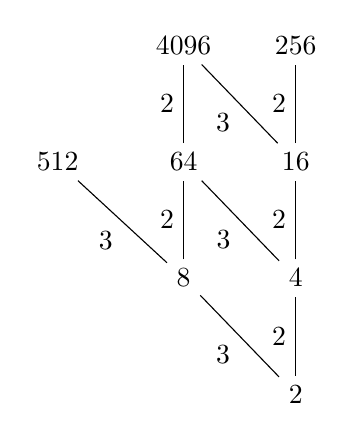
\begin{tikzpicture}
    \node (2) {$\finitefield{2}$};
    \node (4) [above = of 2] {$\finitefield{4}$};
    \node (16) [above = of 4] {$\finitefield{16}$};
    \node (256) [above = of 16] {$\finitefield{256}$};

    \node (8) [above left = of 2] {$\finitefield{8}$};
    \node (64) [above = of 8] {$\finitefield{64}$};
    \node (4096) [above = of 64] {$\finitefield{4096}$};
    
    \node (512) [above left = of 8] {$\finitefield{512}$};

    \path
      (2) edge node[auto] {2} (4)
      (4) edge node[auto] {2} (16)
      (16) edge node[auto] {2} (256)
      (2) edge node[auto] {3} (8)
      (4) edge node[auto] {3} (64)
      (16) edge node[auto] {3} (4096)
      (8) edge node[auto] {2} (64)
      (64) edge node[auto] {2} (4096)
      (8) edge node[auto] {3} (512);
  \end{tikzpicture}
\end{figure}
The union of all these fields is $\overline{\finitefield{p}}$, and we have:
\begin{equation*}
  \finitefield{q} = \{ x \in \overline{\finitefield{q}} \mid x^q = x \} \text{ for } q = p^n
\end{equation*}

\begin{lemma}
  \label{lemma:66}
  Consider a finite extension $\finitefield{q^n}/\finitefield{q}$. Then the Frobenius map\index{Frobenius map} $\text{Fr}_q : x \mapsto x^q$ is a $\finitefield{q}$-automorphism of $\finitefield{q^n}$ with order $n$, i.e. 
  \begin{equation*}
    \{ \text{id}, \text{Fr}_q, \text{Fr}_q^2, \ldots, \text{Fr}_q^{n-1} \} \subseteq \autset[\finitefield{q}]{\finitefield{q^n}} \}
  \end{equation*}
\end{lemma}

\begin{proof}
  The map $\text{Fr}_q$ fixes all elements in $\finitefield{q}$ (the roots of $X^q-X$, hence is a $\finitefield{q}$-homomorphism. Being an injective map (by lemma \ref{lemma:11}) of a finite set $\finitefield{q^n}$ into itself, it is a $\finitefield{q}$-automorphism. Since $\forall x \in \finitefield{q^n}$, $x^{q^n}=x$, we have $\text{Fr}_q^n = \text{id}$ on $\finitefield{q^n}$, i.e. the order of $\text{Fr}_q$ in $\autset[\finitefield{q}]{\finitefield{q^n}}$ divides $n$. But, for each $m \mid n$, the elements fixed by $\text{Fr}_q^m$ are exactly the elements in $\finitefield{q^m}$, so the order is $n$.
\end{proof}

\subparagraph{Remark}

For a non-finite K with $\mchar K = p$, the Frobenius map is injective but not necessarily an automorphism (e.g. $\text{Fr} : \finitefield{p}(X) \rightarrow \finitefield{p}(X)$ has image $\finitefield{p}(X^p)$, where $\finitefield{p}(X)$ denotes the field of rational functions). 

\begin{lemma}
  \label{lemma:67}
  Let K be a field, and $K^{\times} = K \setminus \{ 0 \}$ be its multiplicative group. Then every finite subgroup $G$ of $K^{\times}$ is cyclic.
\end{lemma}

\begin{proof}
  Let $x \in G$ be an element with the maximal order, $n$ say. We show that for any $y \in G$, its order $m$ has to divide $n$. Suppose not, then there exists a $p$ prime such that $m = p^jm'$, $n = p^kn'$, and $j > k$ (with $p \nmid m', n'$).

  Let $z = x^{p^k}y^{m'}$, then we have:
  \begin{IEEEeqnarray*}{rCl}
    z^i = 1 &\Rightarrow& x^{{p^k}i} = y^{-im'} \\
    &\Rightarrow&
    \begin{cases}
      x^{p^jp^ki} = y^{-im} = 1 \Rightarrow n \mid p^{j+k}i \Rightarrow n' \mid i \\
      1 = x^{ni} = y^{-im'n'} \Rightarrow m \mid im'n' \Rightarrow p^j  \mid i
    \end{cases} \\
    &\Rightarrow& p^jn' \mid i
  \end{IEEEeqnarray*}
i.e. the order of $z$ is $p^jn' > n$, hence contradiction. Now $x^{in/m}$ ($ 1 \leq i \leq m$) are in distinct roots of $X^m -1$ in K, hence all the roots (lemma \ref{lemma:53}). As $y$ is a root, it is a power of $x$.
\end{proof}

\begin{theorem}
  \label{thm:68}
  Every finite extension $\finitefield{q'}/\finitefield{q}$ is simple and Galois with:
  \begin{equation*}
    \Gal{\finitefield{q^n}/\finitefield{q}} = \{ \text{id}, \text{Fr}, \text{Fr}_q^2, \ldots,  \text{Fr}_q^n \} \cong C_n
  \end{equation*}
\end{theorem}

\begin{proof}
  By lemma \ref{lemma:67}, $\finitefield{q^n}^\times = \finitefield{q^n} \setminus \{ 0 \}$ is cyclic, i.e. $\finitefield{q}^n  = \{ 0, 1, \zeta, \zeta^2, \ldots, \zeta^{q^n-2} \}$ for some $\zeta \in \finitefield{q^n}$, hence $\finitefield{q^n} = \finitefield{q}(\zeta)$ is simple. If $P_\zeta$ is the minimal polynomial of $\zeta$ over $\finitefield{q}$, then:
  \begin{equation*}
    \card{\autset[\finitefield{q}]{\finitefield{q^n}}} \leq \card{\homset[\finitefield{q}]{\finitefield{q^n}}{\finitefield{q^n}}} = \card{\rootset[P_\zeta]{\finitefield{q^n}}} \leq n
  \end{equation*}
by prop \ref{prop:14}. Now lemma \ref{lemma:66} implies the rest.
\end{proof}

\subparagraph{Remark}

Theorem \ref{thm:68} and proposition \ref{prop:14} imply that conjugates of $\zeta$ are:
\begin{equation*}
  \{ \text{Fr}_q^i(\zeta) = \zeta^{q^i} \mid 0 \leq i \leq n-1 \}
\end{equation*}
i.e.
\begin{equation*}
  P_\zeta = (X-\zeta)(X-\zeta^q)(X-\zeta^{q^i})\cdots(X-\zeta^{q^{n-1}})
\end{equation*}
with $\deg P_\zeta = [\finitefield{q^n} : \finitefield{q}]$.

\subparagraph{Example}

Not all generators $\zeta$ of the group $\finitefield{q^n}^\times$ are conjugate over $\finitefield{q}$. For example, in $\finitefield{2}[X]$:
\begin{equation*}
  X^16 - X = \underbrace{\underbrace{X(X+1)}_{\finitefield{2}}(X^2+X+1)}_{\finitefield{4}}\underbrace{(X^4+X^3+X^2+1)(X^4+X+1)(X^4+X^3+1)}_{\text{roots all generate } \finitefield{16}/\finitefield{2}}
\end{equation*}
whose roots are all elements in $\finitefield{2}$. The 8 last roots are generators of $\finitefield{16}^\times \cong C_{15} \cong C_3 \times C_5$ by lemma \ref{lemma:67}.


%%% Local Variables: 
%%% mode: latex
%%% TeX-master: "Galois"
%%% End: 

\section{Hypothesis testing}
\label{sec:3.7}

As before, we suppose a linear model $\vec{Y} = X \vec{\beta} + \vec{\epsilon}$ with normal theory assumptions.
Suppose additionally that we have
\[
X_{n \times p} = \big( {X_0}_{n \times p_0} \mid {X_1}_{n \times (p - p_0)} \big)
\]
and
\[
\vec{\beta}_{p \times 1} =\begin{pmatrix}\vec{\beta_0} \\ \vec{\beta_1}\end{pmatrix} \mpunct{.}
\]
We want tot test $H_0 : \vec{\beta_1} = \vec{0}$ against $H_1 : \vec{\beta_1} \neq \vec{0}$.

Under $H_0$, we have that $\vec{Y} = X_0 \vec{\beta_0} + \vec{\epsilon}$, hence the m.l.es of $\vec{\beta_0}$ and $\sigma^2$ are
\[
\hat\hat{\vec{\beta_0}} = (X_0^TX_0)^{-1} X_0^T Y
\]
and
\[
\hat\hat{\sigma}^2 = \frac{1}{n} \mathrm{RSS}_0 = \frac{1}{n}(\vec{Y} - X_0 \hat{\hat{\vec{\beta_0}}})^T(\vec{Y} - X_0 \hat{\hat{\vec{\beta_0}}}) \mpunct{.}
\]
The fitted values under $H_0$ are
\[
\hat{\hat{\vec{Y}}} =  X_0 (X_0^T X_0) ^{-1} X_0 ^T \vec{Y} = P_0 \vec{Y} \text{ say,}
\]
where $P_0 = X_0(X_0^TX_0)^{-1}X_0^T$.

Under $H_1$, the m.l.es are $\hat{\beta} = (X^TX)^{-1}X^T\vec{Y}$ and $\hat{\sigma}^2 = \mathrm{RSS}/n$.

The generalised likelihood ratio of $H_0$ and $H_1$ is
\begin{IEEEeqnarray*}{rCl}
\Lambda_{\vec{Y}}(H_0 ; H_1) &=& \frac{\left(\frac{1}{\sqrt{2 \pi \hat{\sigma}^2}}\right)^n \exp \left \{ - \frac{1}{2 \hat{\sigma}^2} (\vec{Y} - X \hat{\vec{\beta}})^T(\vec{Y} - X \hat{\vec{\beta}}) \right \}}{\left(\frac{1}{\sqrt{2 \pi \hat{\hat{\sigma}^2}}}\right)^n \exp \left \{ - \frac{1}{2 \hat{\hat{\sigma}^2}} (\vec{Y} - X_0 \hat\hat{{\vec{\beta_0}}})^T(\vec{Y} - X_0 \hat{\hat{\vec{\beta_0}}}) \right \}} \\
&=& \left( \frac{\hat{\hat{\sigma}}^2}{\hat{\sigma}^2} \right)^{n/2} \\
&=& \left( \frac{\mathrm{RSS}_0}{\mathrm{RSS}} \right)^{n/2} \\
&=& \left( 1 + \frac{(\mathrm{RSS}_0 - \mathrm{RSS})}{\mathrm{RSS}} \right)^{n/2} \mpunct{.}
\end{IEEEeqnarray*}
We reject $H_0$ when $2 \log \Lambda$ is large, equivalently when $(\mathrm{RSS}_0 - \mathrm{RSS})/\mathrm{RSS}$ is large.

We have $\mathrm{RSS} = \vec{Y}^T(I - P)\vec{Y}$ (see the proof of \cref{thm:3.7}).
We have that
\begin{IEEEeqnarray*}{rCl}
\mathrm{RSS}_0 - \mathrm{RSS} &=& \vec{Y}^T(I - P_0)\vec{Y} - \vec{Y}^2(I - P)\vec{Y} \\
&=& \vec{Y}^T (P - P_0) \vec{Y} \mpunct{.}
\end{IEEEeqnarray*}
$I - P$ and $P - P_0$ are symmetric and idempotent.
We have that
\[
\mathop{rank} P = n -p
\]
by \cref{thm:3.7}, and that
\begin{IEEEeqnarray*}{rCl}
\mathop{rank} (P - P_0) &=& \mathop{tr} (P - P_0) \\
&=&  \mathop{tr} P - \mathop{tr} P_0 \\
&=& \mathop{rank} P - \mathop{rank} P_0 \mpunct{.}
\end{IEEEeqnarray*}
We have further that
\begin{IEEEeqnarray*}{rCl}
(I - P)(P - P_0) &=& (I - P)P - (I - P)P_0 \\
&=& 0 - P_0 - P P_0 \\
&=& 0
\end{IEEEeqnarray*}
Finally, we have that
\[
\vec{Y}^T(I - P)\vec{Y} = (\vec{Y} - X_0 \vec{\beta}_0)^T(I - P)(\vec{Y} - X_0 \vec{\beta}_0)
\]
as we know that $(I - P)X_0 \vec{\beta}_0 = 0$, and that
\[
\vec{Y}^T(P - P_0) \vec{Y} = (\vec{Y} - X_0\vec{\beta}_0)^T(P - P_0)(\vec{Y} - X_0 \vec{\beta}_0)
\]
as we have that $(P - P_0)X_0\vec{\beta}_0$.

Now applying \cref{lemma:3.5} and \cref{lemma:3.8} to
\[
\vec{Z} = \vec{Y} - X_0 \vec{\beta}_0 \quad A_1 = I - P \quad A_2 = P - P_0
\]
to see that, \emph{under $H_0$}, $\vec{Y}^T(I - P)\vec{Y}$ and $\vec{Y}^T(P - P_0)\vec{Y}$ are independent $\sigma^2\chi^2_{n-o}$ and $\sigma^2\chi^2_{p - p_0}$ respectively.
Hence under $H_0$, we have that
\[
F = \frac{\vec{Y}^T(P - P_0)\vec{Y} / (p - p_0)}{\vec{Y}^T (I - P)\vec{Y} / (n - p)} = \frac{(\mathrm{RSS}_0 - \mathrm{RSS})/(p - p_0)}{\mathrm{RSS}/(n- p)} \sim F_{p-p_0, n - p} \mpunct{.}
\]
For a size $a$ test of $H_0$ vs $H_1$, we reject $H_0$  when
\[
F > F_{p - p_0, n - p}(\alpha) \mpunct{.}
\]
$\mathrm{RSS}_0 - \mathrm{RSS}$ is the ``reduction in residual sum of squares due to fitting $\vec{\beta}_1$''.
Note that the above can be extended to more complex $H_0$.

\emph{see examples on sheet}

%%% Local Variables:
%%% mode: latex
%%% TeX-master: "statistics"
%%% End:


\subparagraph{Remark}

\begin{enumerate}
\item Later we will see another ``mod p proof'', i.e. proving that $\Gal{P}$ for $P \in \mathbb{Q}[X]$ is large by showing $\Gal{P \mod p}$ is large for some $p$. (see theorem \ref{thm:84}).

\item Let $N = 8$, $\zeta = \zeta_8$, $\Phi_8 = (X-\zeta)(X-\zeta^3)(X-\zeta^5)(X-\zeta^7)$.
  \begin{figure}[H]
    \centering
    \begin{tikzpicture}
      \draw (0,0) circle (2cm);
      \draw (-2.5cm, 0) -- (2.5cm, 0);
      \draw (0, -2.5cm) -- (0, 2.5cm);
      \foreach \a in {1, 3, 5, 7}
      {
        \draw (\a*45:1.85cm) -- (\a*45:2.15cm);
        \node at (\a*45:2.4cm) {$\zeta^{\a}$};
      }
    \end{tikzpicture}
  \end{figure}
 By building the theory of number fields and reducing $\mathbb{Z}[\zeta]$ modulo $p$ to get $\finitefield{p}(\unityroots{N}) \ni \overline{\zeta} = ``\zeta \mod p''$. (in fact, this is a natural way to obtain all finite extensions of $\finitefield{p}$). One sees from the remark after theorem \ref{thm:68} that the factorization of $\overline{\Phi_8} = \Phi_8 \mod p$ in $\finitefield{p}[X]$ is as:
  \begin{description}
  \item[$p \equiv 1 \mod 8$: ] 
\[
\overline{\Phi_8} = \left(X - \overline{\zeta}\right)\left(X - \overline{\zeta}^3\right)\left(X - \overline{\zeta}^5\right)\left(X - \overline{\zeta}^7\right)
\]
  \item[$p \equiv 3 \mod 8$: ] 
\[
\overline{\Phi_8} = \left[\left(X-\overline{\zeta}\right)\left(X-\overline{\zeta}^3\right)\right]\left[\left(X-\overline{\zeta}^5\right)\left(X-\overline{\zeta}^7\right)\right]
\]
\[
\text{e.g.} \ p = 3, \ (\Phi_8 \mod 3) = \left(X^2+X-1\right)\left(X^2-X-1\right)
\]
  \item[$p \equiv 5 \mod 8$: ] 
\[
\overline{\Phi_8} = \left[\left(X-\overline{\zeta}\right)\left(X-\overline{\zeta}^5\right)\right]\left[\left(X-\overline{\zeta}^3\right)\left(X-\overline{\zeta}^7\right)\right]
\]
\[
\text{e.g.} \ p = 5, \ (\Phi_8 \mod 5) = \left(X^2-2\right)\left(X^2+2\right)
\]
  \item[$p \equiv 7 \mod 8$: ] \ldots
\[
\text{e.g.} \ p = 7, \ (\Phi_8 \mod 7) = \left(X^2 + 3X + 1\right)\left(X^2-3X+1\right)
\]
  \end{description}
which explains why $\Phi_8$ is irreducible in $\mathbb{Q}[X]$: if it were factorized in $\mathbb{Z}[X]$ (say into $(X-\zeta)(X-\zeta^3)$ etc.), every mod $p$ reduction must respect this.

\item Theorem \ref{thm:71} says $\mathbb{Q}(\unityroots{N})/\mathbb{Q}$ has Galois group $\multCyclicGp{N}$, an abelian group of order $\varphi(N) = \{ i \mod N \mid 1 \leq i \leq N, (i, N) = 1 \}$ (where $\varphi$ denotes Euler's function\index{Euler's function}). If $N = \prod_i p_i^{m_i}$, then $\varphi(N) = \prod_i \varphi(p_i^{m_i})$, and $\varphi(p^m) = p^{m-1}(p-1)$ for $p$ prime. Revisit the ruler and compass construction of a regular N-gon, i.e. points in $\mathbb{Q}(\unityroots{N})$, is constructible if and only if $[\mathbb{Q}(\unityroots{N}) : \mathbb{Q}] = \varphi(N)$ is a power of 2, if and only if $N = 2^ap_1p_2\cdots{}p_r$, where $p_i$ are distinct Fermat primes, e.g. $p = 17$ (Gauss, c.f. example sheet 2.10).
  \begin{figure}[H]
    \centering
    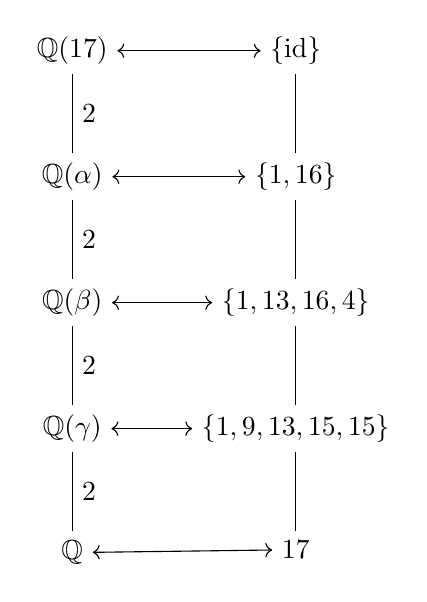
\begin{tikzpicture}
      \node (1) {$\mathbb{Q}(\unityroots{17})$};
      \node (2) [below = of 1] {$\mathbb{Q}(\alpha)$};
      \node (3) [below = of 2] {$\mathbb{Q}(\beta)$};
      \node (4) [below = of 3] {$\mathbb{Q}(\gamma)$};
      \node (5) [below = of 4] {$\mathbb{Q}$};

      \node (6) [right = 0.15\linewidth  of 1] {$\{ \text{id} \}$};
      \node (7) [below = of 6] {$\{ 1, 16 \}$};
      \node (8) [below = of 7] {$\{ 1, 13, 16, 4 \}$};
      \node (9) [below = of 8] {$\{ 1, 9, 13, 15, 15 \}$};
      \node (10) [below = of 9] {$\multCyclicGp{17}$};

      \path
        (1) edge node[auto] {2} (2)
        (2) edge node[auto] {2} (3)
        (3) edge node[auto] {2} (4)
        (4) edge node[auto] {2} (5);

      \path 
        (6) edge node {} (7)
        (7) edge node {} (8)
        (8) edge node {} (9)
        (9) edge node {} (10);

      \foreach \s/\t in {1/6, 2/7, 3/8, 4/9, 5/10}
      {
        \path (\s) edge[<->] node {} (\t);
      }
    \end{tikzpicture}
  \end{figure}
Let $\zeta = \zeta_{17}$, and $\alpha = \zeta + \zeta^{16} = 2\cos \frac{2\pi}{17}$, $\alpha' = \zeta^{13} + \zeta^4$ are roots of $X^2 -\beta_1X + \beta_3$, where $\beta = \beta_1 = \zeta + \zeta^{13} + \zeta^{16} + \zeta^4$, and $\beta_2 = \zeta^9 + \zeta^{15} + \zeta^8 + \zeta^2$ are roots of $X^2  -\gamma{}X - 1$, and $\beta_3$, $\beta_4$ are roots of $X^2 -\gamma'X-1$, with $\gamma = \zeta + \zeta^9 + \cdots + \zeta^2$ (8 terms), and $\gamma' = \zeta^3 + \zeta^{10} + \cdots$ (the rest). Hence $\gamma + \gamma' = 1$, $\gamma\gamma' = -4$, thus $\gamma = \frac{-1 + \sqrt{17}}{2}$.
\end{enumerate}

\section{Separability}

\begin{definition}
\label{def:72}
  Let $K$ be a field. A polynomial $P \in K[X]$ is called separable\index{separable} if $\card{\rootset[P]{E}} = \deg P$ (i.e. no multiple root) whenever P splits in an extension $E/K$ (by lemma \ref{lemma:55}, $\card{rootset{E}}$ independent of $E$).
\end{definition}

\begin{lemma}
\label{lemma:73}
\begin{enumerate}
\item Let $L/K$ be an extension. If $P$ is separable and $Q \in L[X]$ divides $P$ in $L[X]$ then $Q$ is separable.
\item $P$ is separable if and only if $P$ and $D(P)$ are coprime in $K[X]$.
\item If $P$ is irreducible, then $P$ is separable if and only if $D(P) \neq 0$, i.e.$P$ is not a polynomial in $X^p$ for $p = \mchar K$. In particular, all irreducible polynomials are separable if $\mchar K = 0$.
\item Suppose $P$ is separable. If $\tau : K \hookrightarrow E$ is a field homomorphism then $\tau{}P \in E[X]$ is separable. In particular, $P$ is separable as a polynomial in $L[X]$ for any extensions $L/K$.
\end{enumerate}
\end{lemma}

\begin{proof}
  \begin{enumerate}
  \item As $P$ has no multiple root when split, neither does $Q$. 
  \item Let E be a splitting field of $P$. If $P$, $D(P)$ are coprime, then $\exists Q, R \in K[X]$ with $PQ + D(P)R = 1$ in $K[X]$ (recall prop \ref{prop:15}), which remains true in $E[X]$, so $P$, $D(P)$ have no common root in E. If $P$ and $D(P)$ had a common factor in $K[X]$, then they have a common root in E, hence a multiple root.
  \item As $\deg D(P) < \deg P$ and $P$ irreducible, $P$ and $D(P)$ are coprime unless $D(P) = 0$. 
  \item $\tau{}P$ and $\tau{}D(P) = D(\tau{}P)$ are coprime in $E[X]$ (send $PQ + D(P)R = 1$ by $\tau$).
  \end{enumerate}
\end{proof}

%%% Local Variables: 
%%% mode: latex
%%% TeX-master: "Galois"
%%% End: 

\begin{definition}
  \label{def:74}
  An algebraic extension $F/K$ is called separable\index{separable} (resp. normal\index{normal}), if for every $\alpha \in F$ its minimal polynomial $P_\alpha$ is separable (resp. splits in F).
\end{definition}

We relate the separability with the K-homomorphisms in 1.5. 

\begin{lemma}
  \label{lemma:75}
  Let $F/K$, $E/K$ be two extensions of $K$. Let $K \subseteq L \subseteq F$ and $\alpha \in F$ be algebraic over L with minimal polynomial $P_\alpha$ over L. Then, we have
\[
\card{\homset{L(\alpha)}{E}} \leq \deg P_\alpha \card{\homset{L}{E}}
\]
where the equality holds if and only if $\card{\rootset[\tau{}P_\alpha]{E}} = \deg P_\alpha$ for all $\tau \in \homset{L}{E}$.
\end{lemma}

\begin{proof}
  Immediate from \ref{prop:17}, which gives a bijection for every $\tau \in \homset{L}{E}$.
\begin{IEEEeqnarray*}{rCl}
\{ \rho \in \homset{L(\alpha)}{E} \mid \restr{\rho}{L} = \tau &\rightarrow& \rootset[\tau{}P_\alpha(E)]{E} \\
\rho & \mapsto& \rho(\alpha)
\end{IEEEeqnarray*}
\end{proof}

\begin{proposition}
  \label{prop:76}
  If $F/K$ is finite then $\card{\homset{F}{E}} \leq [F : K]$ for any extension $E/K$. If the equality holds for $E/K$, then for any intermediate field $K \subseteq L \subseteq F$ we have:
\begin{enumerate}
\item $\card{\homset{L}{E}} = [L : K]$
\item
  \begin{IEEEeqnarray*}{rCl}
    \homset{F}{E} & \rightarrow & \homset{L}{E} \\
    \rho & \mapsto & \restr{\rho}{L}
  \end{IEEEeqnarray*}
is surjective.
\end{enumerate}
\end{proposition}
\begin{proof}
  Let $F = K(\alpha_1, \ldots, \alpha_n)$ (by prop \ref{prop:10}), and $K_i = K(\alpha_1, \ldots, \alpha_i)$ so that $K = K_0 \subseteq K_1 \subseteq \cdots \subseteq K_n = F$ is a tower of simple extensions. By repeating lemma \ref{lemma:75} we have:
  \begin{IEEEeqnarray*}{rCl}
    \card{\homset{F}{E}} &\leq& [F : K_{n-1}] \card{\homset{K_{n-1}}{E}} \\
    & \leq & [F : K_{n-1}][K_{n-1} : K_{n-2}] \cdots [K_{i+1} : K_i] \card{\homset{K_i}{E}} \\
    & \leq & [F : K]
  \end{IEEEeqnarray*}
If the equality holds, every $\leq$ has to be an equality. For $K \subseteq L \subseteq F$, choose $\alpha_1, \ldots, \alpha_n$ so that $L = K_i$. Then $[F : L]\card{\homset{L}{E}} = [F : K]$, hence (i) by the tower law, and the condition in lemma \ref{lemma:75} shows that the LHS of (star) is different from $\phi$ for every step from $L = K_i$ to $F_i$ hence (ii)
\end{proof}

\begin{theorem}
  \label{thm:77}
  Let $F/K$ be a finite extension. Then we have that:
  \begin{enumerate}
  \item The following are equivalent:
    \begin{enumerate}
    \item There exists an extension $E/K$ with $\card{\homset{F}{E}} = [F : K]$
    \item $F/K$ is separable
    \item $F = K(\alpha_1, \ldots, \alpha_n)$ and the minimal polynomial $Q_i$ of $\alpha_i$ over K is separable (for $1 \leq i \leq n$)
    \item $F = K(\alpha_1, \ldots, \alpha_n)$ and the minimal polynomial $P_i$ of $\alpha_i$ over $F = K(\alpha_1, \ldots, \alpha_{i-1})$ is separable (for $1 \leq i \leq n$)
    \end{enumerate}
  \item If $K \subseteq L \subseteq F$, then $F/K \ \text{separable} \Leftrightarrow F/L, \, L/K \ \text{separable}$.
  \item The following are equivalent:
    \begin{enumerate}
    \item $F/K$ is Galois
    \item $F/K$ is separable and normal
    \item $F = K(\alpha_1, \ldots, \alpha_n)$ and the minimal polynomial $Q_i$ of $\alpha_i$ over K is separable and splits in $F$ (for $1 \leq i \leq n$).
    \end{enumerate}
  \end{enumerate}
\end{theorem}

\begin{proof}
  (i)
  \begin{description}
  \item[$a \Rightarrow b$] For every $\alpha \in F$, we have:
\[
\card{\rootset[P_\alpha]{E}} = \card{\homset{K(\alpha)}{E}} = [K(\alpha) : K] = \deg P_\alpha
\] where the first equality is by proposition \ref{prop:14} and the second by proposition \ref{prop:76}.
  \item[$b \Rightarrow c$] Trivial.
  \item[$c \Rightarrow d$] $P_i \mid Q_i$, so use lemma \ref{lemma:73}
  \item[$d \Rightarrow a$] Take $E/K$ such that $Q_1$, \ldots, $Q_n$ splits in $E$. We show that every inequality in the proof of proposition \ref{prop:76} is an equality by checking the condition in lemma \ref{lemma:75}. For every $\tau \in \homset{K_{i-1}}{E}$, we have $\tau{}P_i$ separable by lemma \ref{lemma:73}. As $\tau{}P_i \mid \tau{}Q_i = Q_i$ and $Q_i$ splits in E, then $\card{\rootset[\tau{}P_i]{E}} = \deg P_i$.

(ii)
Choose $\alpha_1$, \ldots, $\alpha_n$ with $L = K_i$, and use $b \Leftrightarrow d$ in (i)

(iii) Same proof as (i), in which we can take $E$ to be $F$ everywhere.
  \end{description}
\end{proof}
Now we revisit paragraphs 1.5-1.7. For every finite separable $F/K$, the assertions theorem \ref{thm:18} and lemma \ref{lemma:19} hold with $\mathbb{C}$ replaced by some field $E$, by theorem \ref{thm:77}(i)(a) and proposition \ref{prop:76}(ii).

\begin{theorem}[Primitive element theorem]
\label{thm:78}
  Every finite separable extension is simple.
\end{theorem}
\begin{proof}
  By theorem \ref{thm:77} and proposition \ref{prop:76}, the condition (star) in the proof of theorem \ref{thm:20} holds.
\end{proof}

\begin{proposition}
  \label{prop:79}
  The following unconditionally (i.e. without the restriction of being a subfield of $\mathbb{C}$).
  \begin{itemize}
  \item lemma 22 (iii), corollary 26, with the condition that ``$P$ is a product of separable polynomials''.
  \item proposition 33
  \item theorem 34 (FTGT)
  \item corollary 35
  \item proposition 42
  \end{itemize}
\end{proposition}
\begin{proof}
  Lemma 22(iii) is a special case of proposition 76. Theorem 77(iii) corresponds to proposition 24, and the rest follows. In the proof of corollary 35, proposition 42, replace $\mathbb{C}$ with F, and use proposition 76 for $E = F$.
\end{proof}

For example, applying proposition \ref{prop:42} to finite fields gives:
\begin{proposition}
  \label{prop:80}
Let $P \in \finitefield{p}[X]$ be a monic separable polynomial of degree $n$. If = $P = Q_1\cdots{}Q_m$ is the irreducible factorization in $\finitefield{p}[X]$ with $\deg Q_i = n_i$ (so $n = \sum n_i$), then $\operatorname{Fr_p} \in \Gal{P} \hookrightarrow S_n$ has cycle type $(n1, \ldots, n_m)$ when viewed as an element of $S_n$.
\end{proposition}

\subparagraph{Remark}

$\Gal{P} \hookrightarrow S_n$ is defined up to conjugation in $S_n$, hence the cycle type is well-defined.

\begin{proof}
  Let $\finitefield{q}$ be the splitting field of $P$ over $\finitefield{p}$. As $\Gal{\finitefield{q}/\finitefield{p}} = \{ \operatorname{id}, \operatorname{Fr}_p, \operatorname{Fr}_p^2, \ldots, \operatorname{Fr}_p^{N-1} \}$ if $q = p^N$ (by theorem \ref{thm:68}, the conjugates of $\alpha$ over $\finitefield{p}$ are $\{ \alpha, \alpha^p, \alpha^{p^2}, \ldots, \alpha^{p^{N-1}} \}$ for some $d \mid N$, which are permuted cyclically by $\text{Fr}_p$. Now $P = Q_i\cdots{}Q_m$ and each $Q_i$ being irreducible, is the minimal polynomial of its root $\alpha_i \in \finitefield{q}$. So in $\finitefield{q}[X]$, we have that
  \begin{IEEEeqnarray*}{rlr}
    P = & (X-\alpha_1)(X-\alpha_1^p)\cdots{}(X - \alpha_1^{p^{n_1-1}}) & \leftarrow Q_1 \\
    & (X-\alpha_2)(X-\alpha_2^p)\cdots(X-\alpha_2^{p^{n_2-1}}) & \leftarrow Q_2 \\
    & \cdots{}(X-\alpha_m)\cdots{}(X-\alpha_m^{p^{n_m-1}}) & \leftarrow Q_m
  \end{IEEEeqnarray*}
and $\operatorname{Fr}_p$ acts on these n roots by a permutation of cycle type $(n_1, \ldots, n_m)$.
\end{proof}

%%% Local Variables: 
%%% mode: latex
%%% TeX-master: "Galois"
%%% End: 


\section{Example II: Symmetric function theorem}

Let $K$ be a field and $n \geq 1$. Recall \autoref{def:43}: $F = K(X_1, \ldots, X_n)$ the field of rational functions in $n$ variables (the field of fractions of $K[X_1, \ldots, X_n]$. As used in the proof of \autoref{prop:42}, the symmetric group $G = S_n$ acts on $F$ by permuting $X_1$, \ldots, $X_n$, i.e. $G \subseteq \autset[K]{F}$. The fixed field $F^G$ is the subfield consisting of all symmetric rational functions in $X_1$, \ldots, $X_n$.

\begin{definition}
  Let $K$n $n$, $F$, $G$ as above. For $1 \leq i \leq n$, let
\[
s_i = \sum_{\{\lambda_1, \ldots, \lambda_i\} \subseteq \{1, \ldots, n \}} X_{\lambda_1}\cdots{}X_{\lambda_i} \in F^G
\]
be the i\textsuperscript{th} elementary symmetric polynomial\index{elementary symmetric polynomial}.
\end{definition}

\begin{proposition}[Rational symmetric function theorem]
   Let $K$n $n$, $F$, $G$ as above, and let $L = K(s_1, \ldots, s_n) \subseteq F$ be the subfield of F consisting of all rational functions in $s_1$, \ldots, $s_n$ with coefficient in K. Then, we have that $L = F^G$, i.e. all symmetric functions are in $L$.
\end{proposition}

\begin{proof}
  As $s_1, \ldots, s_n \in F^G$ we have $L \subseteq F^G$. As $X_1$, \ldots, $X_n$ are the roots of $P(X) = (X-X_1)\cdots{}(X-X_n) = X^n-s_1X^{n-1}+s_2X^{n-2}-\cdots{}+(-1)^ns_n \in L[X]$. $F = L(X_1, \ldots, X_n)$ is a splitting field of P, finite over L.So $F/F^G$ is also finite.

\paragraph{Path I}
 \autoref{prop:33} says $F/F^G$ is Galois with $G = \Gal{F/F^G}$. As $F$ is a splitting field of $P$ over $L$, and $P$ has no multiple roots, hence $F/L$ is also Galois, and $\Gal{P} = \Gal{F/L}$ injects to $G$ (permutation of the $X_i$) by \autoref{prop:79}. Thus $F^G = L$ follows from:
\[
\card{G} = \card{\Gal{F/F^G}} = [F : F^G] \leq [F : L] = \card{\Gal{F/L}} \leq \card{G}
\]
hence we have equality.

\paragraph{Path II}

We build from first principles. As $G \subseteq \autset[F^G]{F}$, we have:
\[
n! = \card{G} \leq \card{\autset[F^G]{F}} \leq [F : F^G] \leq [F : L] \label{eq:asterisk} \tag{*}
\]
but a splitting field has degree at most $n!$. Let $L_i = L(X_1, \ldots, X_i)$ for $1 \leq i \leq n$, so that $L = L_0 \subseteq L_1 \subseteq L2 \subseteq \cdots \subseteq L_n = F$. Then $X_i$ is a root of:
\[
P_i(X) = \frac{P(X)}{(X-X_1)\cdots{}(X-X_{i-1})} = (X-X_i)\cdots{}(X-X_n) \in L_{i-1}[X] \label{eq:star} \tag{$\star$}
\]
which has degree $n-i+1$, hence $L_i = L_{i-1}(X_i)$ has at most degree $n-i+1$ over $L_{i-1}$. Thus $[F : L] \leq n(n-1)\cdots{}2\cdot{}1 = n!$ by tower law, hence \eqref{eq:asterisk} implies $[F : L] = n!$ and $F^G = L$.
\end{proof}

\paragraph{Remark}

In path II, as $[F : L] = n!$, we need $[L_i, L_{i-1}] = n - i + 1$ for all $i$, i.e. $Z_i = \{ 1, X_i, X_i^2, \ldots, X_i^{n-i} \}$ is a basis of $L_i/L_{i-1}$. Hence:
\[
Z = \{ z_1, \ldots, z_n \mid z_i \in Z_i \} = \{ X_1^{m_1}\cdots{}X_n^{m_n} \mid 0 \leq m_i \leq n-i \}
\]
is a basis of $F/L$ (as seen in the proof of the tower law.

Now revisit \eqref{eq:star} with $n = 3$, $K = \mathbb{Q}$, $(\alpha, \beta, \gamma) = (X_1, X_2, X_3)$ and consider:
\begin{IEEEeqnarray*}{rCl}
  P(X) &=& X^3-(\alpha+\beta+\gamma)X^2 + (\alpha\beta+\beta\gamma+\gamma\alpha)X -\alpha\beta\gamma \\
  &=& P_1(X) \in \mathbb{Z}[s_1, s_2, s_3][X] \\
  &=& (X-\alpha)\underbrace{(X^2-(s_1-\alpha)X + (s_2 -\alpha(s_1-\alpha)))}_{= P_2(X) \in \mathbb{Z}[s_1, s_2, s_3, \alpha, \beta][X]} \\
  &=& (X-\alpha)(X-\beta)\underbrace{(X-(s_1-\alpha-\beta))}_{=P_3(X) \in \mathbb{Z}[s_1, s_2, s_3, \alpha, \beta][X]}
\end{IEEEeqnarray*}

\begin{theorem}[Symmetric function theorem]
  Let $K$, $n$, $F$, $G$ be as above, and let $R$ be any subring of K (e.g. $R = \operatorname{Im} (\mathbb{Z} \rightarrow K)$, i.e. $\mathbb{Z}$ or $\finitefield{Q}$ according to $\mchar K$). Then, inside $F$, we have:
\[
R[X_1, \ldots, X_n] \cap F^G = R[s_1, \ldots, s_n]
\]
i.e. every symmetric polynomial with coefficient in R is a polynomial in $s_1$, \ldots, $s_n$ with coefficient in $R$.
\end{theorem}

\begin{proof}
  Clearly $R[s_1, \ldots, s_n] \subseteq R[X_1, \ldots, X_n] \cap F^G$. In (star), note that $P(X) \in R[s_1, \ldots, s_n][X]$ and $(X-X_1)\cdots{}(X-X_{i-1}) \in R[X_1, \ldots, X_{i-1}][X]$ are both monics with coefficient in the ring $R[s_1, \ldots, s_n, X_1, \ldots, X_i]$, hence by division algorithm we have $P_i(X) \in R[s_1, \ldots, s_n, X_1, \ldots, X_{i-1}][X]$ is a monic polynomial of degree $n-i+1$. As $P_i(X_i) = 0$, we see that $X_i^{n_i+1}$ is a linear combination of $Z_i = \{ 1, X_i^2, \ldots, X_i^{n_i} \}$ over $R[s_1, \ldots, s_n, X_1, \ldots, X_{i-1}]$, hence so is any higher power of $X_i$. Repeating or $1 \leq i \leq n$, eventually every monomial $X_1^{m_1}$, \ldots, $X_n^{m_n}$ is a linear combination of $Z$ over $R[s_1, \ldots, s_n]$, which is a basis of $F/L$. If we write $f \in R[X_1, \ldots, X_n] \cap F^G$ as a linear combination of $Z$ over $R[s_1, \ldots, s_n]$, then it must be the unique expression of $f$ as a $L$-linear combination of $Z$, namely $f = f\cdot{}1$. Thus $f \in R[s_1, \ldots, s_n]$.
\end{proof}

\paragraph{Remark}

The proof shows that $R[X_1, \ldots, X_n]$ is a free $R[s_1, \ldots, s_n]$-module of rank $n!$ with a basis $Z$. We can prove that $R[s_1, \ldots, s_n]$ is isomorphic to the polynomial ring in $s_1$, \ldots, $s_n$ over $R$.

%%% Local Variables: 
%%% mode: latex
%%% TeX-master: "Galois"
%%% End: 


\paragraph{Example}

Recall (\autoref{def:50}) that the discriminant for the splitting field $F = \mathbb{Q}(X_1, \ldots, X_n)$ over $L = \mathbb{Q}(s_1, \ldots, s_n) = F^G$ is:
\[
\Delta{}p = \prod_{i<j}(X_i-X_j)^2 \in \mathbb{Z}[X_1, \ldots, X_n] \cap L = \mathbb{Z}[s_1, \ldots, s_n]
\]
e.g. for $P = X^2 -s_1X + s_2$, we have $\Delta{}p = s_1^2-4s_2$. For $P = X^3 +s_2X-s_3$, we have $\Delta{}p = -4s-2^3-27s_3^2$.

\section{Application II: Galois groups over $\mathbb{Q}$}

\begin{theorem}
\label{thm:84}
  Let $P \in \mathbb{Z}[X]$ be a monic separable polynomial (as $P \in \mathbb{Q}[X]$) of degree $n$, and let $p$ be a prime such that $P \mod p \in \finitefield{p}[X]$ is also separable. If $P \mod p = Q_1\cdots{}Q_m$ is the irreducible factorization in $\finitefield{p}[X]$ and $\deg Q_i = n_i$, then $\Gal{P}$ contains an element with cycle type $(n_1, \ldots, n_m)$ as an element of $S_n$ (see the remark after \autoref{prop:80}).
\end{theorem}

\paragraph{Example}

Let $P = X^5 + 2X + 6$. As $P \mod 3 = X^5-X =  X(X-1)(X+1)(X^2+1)$ in $\finitefield{3}[X]$, \autoref{thm:84} shows that $\Gal{P}$ contains an element of type $(1, 1, 1, 2)$, i.e. a transposition. If moreover $\Gal{P}$ has a 5-cycle, then $\Gal{P} \cong S_5$ by group theory.

\begin{proof}
  By \autoref{prop:80}, suffices to prove that $\Gal{P \mod p} \subseteq \Gal{P}$ inside $S_n$, up to conjugation. We use the setup in (section 2.6, i.e. previous one). Let $F = \mathbb{Q}(X_1, \ldots, X_n)$, on which $G = S_n$ acts by permuting $X_i$, i.e. $\rho(X_i) = X_{\rho(i)}$ for $\rho \in G$. Recall $F^G = \mathbb{Q}(s_1, \ldots, d_n)$ (by \autoref{prop:82}). Let $A = \mathbb{Z}[s_1, \ldots, s_n]$, a subring of $B = \mathbb{Z}[X_1, \ldots, X_n]$. Then \autoref{thm:83} says that $B \cap F^G = A$. Note that the action of $G$ on $F$ restricts to its action on B (permuting $X_i$), and define the 2\textsuperscript{nd} G-action on the ring $B[T_1, \ldots, T_n] = \mathbb{Z}[X_1, \ldots, X_n, T_1, \ldots, T_n]$ by permuting $T_i$ as $\rho(T_i) = T_{\rho(i)}$. We write $\underline{T}$ for $T_1, \ldots, T_n$. Now take a monic of degree $n!$ in $X$ with coefficients in $B[\underline{T}]$:
\[
R = \prod_{\sigma \in G}R_\sigma, \quad R_\sigma = X - \sum_{i=1}^n\sigma(X_i)T_i = X-(X_{\sigma(1)}T_1 + \cdots + X_{\sigma(n)}T_n) \in B[\underline{T}][X]
\]
Then the two actions of $\rho \in G$ permutes the factors $R_\sigma$ as:
\[
R_\sigma \mapsto R_{\rho\sigma} \quad \text{ and } \quad R_\sigma \mapsto R{\sigma\rho^{-1}}
\]
respectively. In particular, the product $R$ is fixed by both actions of $G$. As $R$ is fixed by the first action, so is each coefficient of $T_1^{m_1}\cdots{}T_n^{m_n}X$ (elements in $B$), hence they are in $B \cap F^G = A$. Thus $R \in A[\underline{T}][X]$.

\begin{lemma}
  \label{lemma:85}
  Let $K$ be a field. $ P = X^n - a_1X^{n-1} + \cdots + (-1)^na_n \in K[X]$, and $E/K$ be a splitting field of $P$ over $K$, with $\rootset{E} = \{ \alpha_1, \ldots, \alpha_n \}$. This ordering gives the injection $H = \Gal{P} = \Gal{E/K} \hookrightarrow S_n = G$. Let $A$, $B$, $R$, and $R_\sigma$ as above.

Define a ring homomorphism $\tau : B \rightarrow E$ by $\tau(X_i) = \alpha_i$. Then $\tau{}R \in E[\underline{T}][X]$ lies in $K[\underline{T}][X]$, and its irreducible factorization in $K(\underline{T})[X]$ is given by:
\[
\tau{}R  = \prod_{H\sigma \in H \textbackslash G} \tau{}R_{H\sigma}
\]
where $H\textbackslash{}G$ is the set of right cosets and $R_{H\sigma} = \prod_{\rho \in H\sigma} R_\rho \in B[\underline{T}][X]$. The stabilizer of $\tau{}R_{H\sigma} \in K(\underline{T})[X]$ under the 2\textsuperscript{nd} G-action is $\sigma^{-1}H\sigma$.
\end{lemma}

\begin{proof}
  As $\tau$ is a ring homomorphism, $\tau{}R = \prod_{\sigma \in G} \tau{}R_\sigma$ in $E[\underline{T}][X]$. As $\tau(s_i) = a_i$, we have $\tau(A) \subseteq K$. Since $R \in A[\underline{T}][X]$, we have $\tau{}R \in K[\underline{T}][X]$. For each coset $H\sigma$, the polynomial $R_{H\sigma} \in B[\underline{T}][X]$ is fixed by the 1\textsuperscript{st} action of $H \subseteq G$. Note that the 1\textsuperscript{st} action of $H \subseteq G$ on $X_i$ is sent by $\tau$ to the $H = \Gal{E/K}$-action on $\alpha_i$. Hence $\tau{}R_{H\sigma} \in E[\underline{T}][X]$ is fixed by the action of $H = \Gal{E/K}$. Therefore, so is each coefficient of monomials of $T_1^{m_1}\cdots{}T_n^{m_n}X$ (elements in $E$), thus they are in $E^H = K$ (by \autoref{prop:33}). Hence $\tau{}R = \prod_{H\sigma \in H \textbackslash G}\tau{}R_{H\sigma}$ in $K[\underline{T}][X]$. We show that this is the irreducible factorisation in $K(\underline{T})[X]$. If $Q$ is a monic irreducible factor of $\tau{}R$ in $K(\underline{T})[X]$ such that $\tau{}R_{\sigma} \mid Q$ in $E(\underline{T})[X]$,  then for every $\rho \in H$, we have $\tau{}R_{\rho\sigma} = \tau(\rho(R_\sigma)) = \rho(\tau{}R_\sigma) \mid \rho{}Q = Q$ (as $\restr{\rho}{K} = \text{id}$). As each $\tau{}R_{\rho\sigma}$ is a distinct linear polynomial, their product $\tau{}Ro_{H\sigma}$ must divide $Q$ in $E(\underline{T})[X]$, hence also in $K(\underline{T})[X]$.

Now that the 2\textsuperscript{nd} G-action on $T_i$ is simply sent by $\tau$ to the G-action on $T_i$. Hence $\rho \in G$ sends $\tau{}R_{H\sigma}$ to $\tau{}R_{H\sigma\rho^{-1}$, and $\rho$ fixes it if and only if $\rho \in \sigma^{-1}H\sigma$.
\end{proof}

Now we finish the proof of \autoref{thm:84}. Let $P = X^n - a_1X^{n-1} + \cdots + (-1)^na_n \in \mathbb{Z}[X]$, with its splitting field $E/Q$, and $\rootset[P]{E} = \{ \alpha_1, \ldots, \alpha_n \}$, so that $H = \Gal{P} = \Gal{E/K} \subseteq G$. Define $\tau : B \rightarrow E$ as in \autoref{lemma:85} by $X_i \mapsto \alpha_i$, then $\tau(s_i) = a_i$, hence $\tau{}R \in \mathbb{Z}[\underline{T}][X]$. By Gauss's lemma, the irreducible factorization of $\tau{}R$, monic in $\mathbb{Z}[\underline{T}][X]$, is the same as the irreducible factorization in $\mathbb{Q}(\underline{T})[X]$, since $\mathbb{Z}[\underline{T}]$ is a UFD and $\mathbb{Q}(\underline{T}) = \operatorname{Frac}(\mathbb{Z}[\underline{T}]$. Similarly for $P \mod p \in \finitefield{p}[X]$, let $\finitefield{q}/\finitefield{p}$ be its splitting field with the roots $\beta_1, \ldots, \beta_n \in \finitefield{q}$, so that $H' = \Gal{P \mod p} = \Gal{\finitefield{q}/\finitefield{p} \subseteq G$. Define $\tau': B \rightarrow \finitefield{q}$ by $X_i \mapsto \beta_i$. Then $\tau'(s_i) = a_i \mod p$, hence $\tau'R = \tau{}R \mod p \in \finitefield{p}[\underline{T}][X]$. Its factorization in $\finitefield{q}(\underline{T})[X]$ respects the factorization of $\tau{}R$ in $\mathbb{Z}[\underline{T}][X]$, i.e. each $\tau'R_{H'\sigma} \in \finitefield{p}(\underline{T})[X]$ must divide the mod-p of some $\tau{}R_{H\sigma} \in \mathbb{Z}[\underline{T}][X]$. As the 2\textsuperscript{nd} G-action (permuting $T_i$) is compatible with $\mod p$, the stabilizer $\sigma'^{-1}H\sigma'$ of the former is contained in the stabiliser $\sigma^{-1}H\sigma$ of the latter, hence $H' \subseteq \sigma'\sigma^{-1}H\sigma\sigma^{-1}$.

\end{proof}

%%% Local Variables: 
%%% mode: latex
%%% TeX-master: "Galois"
%%% End: 


\chapter{Modern Galois Theory (Linear Algebra approach)}
\label{chap:3}

Here we rebuild Galois theory using more linear algebra, without ever mentioning polynomials. In this context the principal element theorem is avoided, we only assume the following: \autoref{def:1}, \autoref{def:2}, \autoref{prop:8}, \autoref{def:12}, and from Linear Algebra, \autoref{lemma:11}, \autoref{lemma:22}.

\section{Dedekind's and Artin's lemma}
\label{sec:3.1}

\begin{lemma}
  \label{lemma:86}
  Let $V$ be a finite dimensional vector space over $K$ and $E/K$ an extension. Let $\homset[\text{K-v.s.}]{V}{E}$ be the set of all $K$-linear maps $V \rightarrow E$, and define the addition and $E$-action by:
\[
(\rho + \rho')(x) = \rho(x) + \rho'(x), \ (\alpha\rho)(x)=\alpha\cdot{}\rho(x)
\]
Then it is an $E$-vector space with $\dim_E (\homset[K-\text{v.s.}]{V}{E}) = \dim_K V$.
\end{lemma}

\begin{proof}
  It satisfies the axioms of an $E$-vector space. Let $\{ e_1, \ldots, e_n \}$ be a basis of $V$. If we define $\rho_i \in \homset[K-\text{v.s.}]{V}{E}$ by $\rho_i(a_1e_1 + \cdots{} + a_ne_n) = a_i$, then every $\rho$ is uniquely written as $\rho = \rho(e_1)\rho_1 + \cdots{} + \rho(e_n)\rho_n$ (as we have that $\rho(x) = \rho(\sum_i a_ie_i) = \sum_i a_i\rho(e_i) = \sum_i \rho_i(x)\rho(e_i) \in E$), hence $\{ p_1, \ldots, p_n \}$ is a basis of $\homset[K-\text{v.s.}]{V}{E}$ as an $E$-v.s.
\end{proof}

\begin{proposition}[Dedekind's lemma]
  \label{prop:87}
  \index{Dedekind's lemma}
  Let $F/K$ be a finite extension. Then for any extension $E/K$, the subset $\homset{F}{E}$ of the $E$-vector space $\homset[K-\text{v.s.}]{V}{E}$ is $E$-linearly independent. In particular, $\card{\homset{F}{E}} \leq [F : K]$ (by \autoref{lemma:86}).
\end{proposition}

\paragraph{Remark}

We proved this inequality in \autoref{prop:76}.

\begin{proof}
  We prove that any finite subset $\{ \rho_1, \ldots, \rho_k \}$ of $\homset{F}{E}$ is $E$-linearly independent, by induction on $k$. Let the following $E$-linear relation hold: 
\[
a_1\rho_1 + \cdots + a_k\rho_k = 0 \tag{*} \label{prop:87:asterisk}
\] If $k = 1$, then $\rho_1 \neq 0$ hence $a_1 = 0$, hence the claim holds. Let $k > 1$, for any $x, y \in F$, we have $a_1\rho_1(x)\rho_1(y) + \cdots + a_k\rho_k(x)\rho_k(y) = a_1\rho_1(xy) + \cdots + a_k\rho_k(xy) = 0$. As $y$ is arbitrary, we have equality as a $K$-linear map (i.e. in $\homset[K-\text{v.s.}]{F}{E}$):
\[
a_1\rho_1(x)\rho_1 + \cdots + a_k\rho_k(x)\rho_k = 0
\]
multiply \eqref{prop:87:asterisk} by $p_k(x)$ gives $a_1p_k(x)p_1 + \cdots + a_kp_k(x)p_k = 0$, so subtracting we obtain:
\[
a_1(\rho_1(x)-\rho_k(x))\rho_1 + \cdots + a_{k-1}(\rho_{k-1}(x)-\rho_k(x)) = 0
\]
Then all coefficients are 0 by induction hypothesis, and as $x$ is arbitrary, we have $a_i(\rho_i -\rho_k) = 0$, ($1 \leq i \leq k-1$). If $a_i \neq 0$, then multiplying by $a_i^{-1}$ gives $\rho_i = \rho_k$. Now the case $k = 1$ gives $a_k = 0$.
\end{proof}

This implies $\card{\autset[K]{F}} \leq [F : K]$ for finite $L/K$ (\autoref{lemma:22}). Now recall \autoref{def:23} and \autoref{lemma:32}. Then the first part of \autoref{prop:33} (that $F/K$ Galois implies $F^G = K$) follows. We prove the second part next.

\begin{proposition}[Artin's lemma]
  \label{prop:88}
  Let $F/K$ be any extension. If $G$ is a finite subgroup of $\autset[K]{F}$, then $F/F^G$ is Galois and $\Gal{F/F^G} = G$.
\end{proposition}

\begin{proof}
  Let $G = \{ \rho_1, \ldots, \rho_n\}$ (with $\rho_1 = \text{id}$), and write $\bm{\rho}(x) = \left( \rho_1(x), \rho_2(x), \ldots, \rho_n(x) \right) \in F^n$ for $x \in F$. For $\bm{x} = (x_1, \ldots, x_n) \in F^n$, and $\rho \in G$; write $\rho(\bm{x}) = \big( \rho(x_1), \ldots, \rho(x_n) \big)$. Then $\rho(a\bm{x}) = \rho(a)\rho(\bm{x})$, since $\rho$ is a ring homomorphism, and the components of $\rho(\bm{\rho}(x)) = (\rho\rho_1(x), \ldots, \rho\rho_n(x)) \in F^n$ are a permutation of those $\bm{\rho}(x)$. Hence if we have 
 \[
 a_1\bm{\rho}(x_1) + \cdots + a_k\bm{\rho}(x_k) = 0 \tag{*} \label{prop:88:asterisk}
 \]
 for $a_1, \ldots, a_k \in F$, then by applying $\rho$ to \eqref{prop:88:asterisk} we get:
 \[
 \rho(a_1)\bm{\rho}(x_1) + \cdots + \rho(a_k)\bm{\rho}(x_k) = 0 \tag{$\star$} \label{prop:88:star}
 \]
Now we prove that if $\{x_1, \ldots, x_n\}$ is an $F^G$-linearly independent subset of $F$, then $\{ \bm{\rho}(x_1), \ldots, \bm{\rho}(x_n) \}$ is $F$-linearly independent in $F^n$, which implies $k \leq n  = \card{G}$. Use induction on $k$. If $k = 1$, then $\bm{\rho}(x_i) \neq 0$, since $x_1 \neq 0$, hence the claim holds. Assume an $F$-linear relation \eqref{prop:88:asterisk}. Replacing $a_i$ by $a_i/a_k$ when $a_k \neq 0$, we can assume $a_k + 0$ or $1$. Then as $\rho(a_k) = a_k$ for all $\rho \in G$, \eqref{prop:88:asterisk} - \eqref{prop:88:star} gives:
\[
(a_1 - \rho(a_1))\bm{\rho}(x_1) + \cdots + (a_{k-1} - \rho(a_{k-1}))\bm{\rho}(x_{k-1}) = 0
\]
The induction hypothesis shows that all coefficients are 0, and since $\rho$ was arbitrary, we have $a_i \in F^G$. Now the first component of \eqref{prop:88:asterisk} needs $a_1x_1 + \cdots + a_kx_k = 0$ (as $\rho_1 = \text{id}$), and the $F^G$-linear independence of $\{ x_1, \ldots, x_k \}$ implies all $a_i$ are 0. Thus $F/F^G$ is finite with $[F : F^G] \leq n = \card{G}$. Since we had $\card{G} \leq \card{\autset[F^G]{F}} \leq [F : F^G]$ already, $\card{\autset[F^G]{F}} = [F : F^G]$ and $G = \Gal{F/F^G}$.
\end{proof}

\section{Towers of extensions}
\label{sec:3.2}

We almost reproved the fundamental theorem of Galois (\autoref{thm:34}). Remains to prove that : $K \subseteq L \subseteq F$, $F/K$ Galois implies $F/L$ Galois. To deal with the towers, we generalize the notion of extensions.

\begin{definition}
  \label{def:89}
  Let $K$ be a field. We call a pair $(F, \tau)$ of a field $F$ and a ring homomorphism $\tau : K \rightarrow F$ an extension\index{extension} of $K$, and denote it by $F_\tau$. 

A morphism\index{morphism} $\rho : F_\tau \rightarrow F'_{\tau'}$ of extensions is a ring homomorphism $\rho : F \rightarrow F'$ such that $\rho\tau = \tau'$, i.e. the following diagram commutes.
  \begin{figure}[H]
    \centering
    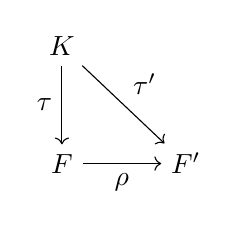
\begin{tikzpicture}
      \node (1) {$K$};
      \node (2) [below = of 1] {$F$};
      \node (3) [right = of 2] {$F'$};

      \path 
        (1) edge[->] node[left] {$\tau$} (2)
        (2) edge[->] node[below] {$\rho$} (3)
        (1) edge[->] node[above right] {$\tau'$} (3);
    \end{tikzpicture}
  \end{figure}
We denote the set of all morphisms from $F_\tau$ to $F'_{\tau'}$ by $\homset[]{F_\tau}{F'_{\tau'}}$. If $\rho$ is bijective, then $\rho^{-1}$ is also a morphism, and we call $\rho$ an isomorphism. An automorphism of $F_\tau$ is an isomorphism from $F_\tau$ to itself, and $\autset[]{F_\tau}$ is the group of all automorphisms of $F_\tau$.
\end{definition}

\paragraph{Remark}

$K$ and $\tau(K)$ are isomorphic (\autoref{lemma:11}, and $F/\tau(K)$ is an extension in our previous definition.

%%% Local Variables: 
%%% mode: latex
%%% TeX-master: "Galois"
%%% End: 


\paragraph{Remark}

If $F_\tau$, $F_{\tau'}$ are extensions in our previous sense (i.e. $\tau$, $\tau'$ are inclusion maps), then $\rho\tau = \tau'$ means $\restr{\rho}{K} = \text{id}$, i.e. morphisms are just K-homomorphisms. Every morphism is injective (\autoref{lemma:11}), and $\tau$ is itself a morphism $\tau : K_{\text{id}} \rightarrow F_\tau$. If $\rho$ is an automorphism of $F_\tau$, then $\restr{\rho}{\tau(K)} = \text{id}$, hence $\autset[]{F_\tau} = \autset[\tau(K)]{F}$. 

\begin{definition}
  \label{def:90}
  Let $F_\tau$ be an extension of a field $K$. We consider $F$ as a vector space over $K$ by letting $x \in K$ act on $F$ via multiplication in $\tau(x)$ in $F$. We say $F_\tau$ is finite if it is a finite dimensional vector space over $K$, and let $[F_\tau] = \dim_K F$ be its degree. A finite extension is called Galois if $\card{\autset[]{F_\tau}} = [F_\tau]$.
\end{definition}

\paragraph{Remark}

We have $[F_\tau] = [F : \tau(K)]$. If $[F_\tau] = 1$, then $\tau$ is bijective and $\tau(K) = F$. Morphisms are injective $K$-linear maps, so $\autset[]{F_\tau} = \homset[]{F_\tau}{F_\tau}$ for finite $F_\tau$ by rank-nullity.

\begin{lemma}
  \label{lemma:91}
  If $\sigma \in \homset[]{F_\tau}{F'_{\tau'}}$, then $\sigma(F)$, $F'$ are extensions of $\tau'(K)$ in our previous sense, and we have a bijection:
  \begin{IEEEeqnarray*}{rCl}
    \homset[\tau'(K)]{\sigma(F)}{F'} &\rightarrow& \homset[]{F_\tau}{F'_{\tau'}}
    \rho & \mapsto & \rho\sigma
  \end{IEEEeqnarray*}
  In particular, if $F_\tau$ is finite then $\card{\homset{F_\tau}{F'_{\tau'}}} \leq [F_\tau]$ by Dedekind (\autoref{prop:87}).
\end{lemma}

\begin{proof}
  (insert diagram 1) In the diagram, $\hookrightarrow$ denotes the inclusion map. As $\restr{\rho}{\tau'(K)} = \text{id}$ implies $\rho\sigma\tau = \tau'$, we have the claimed map. We have the inverse map $\rho' \mapsto \rho'\sigma^{-1}$. Since $\rho'\tau = \tau'$ implies $\restr{\rho'\sigma^{-1}}{\tau'(K)} = \rho'\tau\tau'^{-1} = \text{id}$. If $F_\tau$ is finite, then so is the extension $\sigma(F)_\sigma$ of $\tau(K)$, hence so is $\sigma(F)/\tau'(K)$.
\end{proof}

\begin{definition}
  \label{def:92}
  Let $L_\tau$ be an extension of $K$, and $F_\sigma$ be an extension of $L : K \stackrel{\tau}{\rightarrow} L \stackrel{\sigma}{\rightarrow} F$. Then $\sigma\tau : K \rightarrow F$ is an extension $F_{\sigma\tau}$ of $K$. We cal this a tower $L_\tau$, $F_\sigma$ of extensions.
\end{definition}

\begin{proposition}
  \label{prop:93}
  Let $L_\tau$, $F_\sigma$ be a tower of extensions.
  \begin{enumerate}
  \item If $F'_\tau$ is an extension of $K$, then the set $\homset[]{F_{\sigma\tau}}{F'_{\tau'}}$ is a disjoint union of $\homset[]{F_\sigma}{F'_{\sigma'}}$ for each $\sigma' \in \homset[]{L_\tau}{F'_{\tau'}}$. In particular, $\autset[]{F_\sigma}$ is a subgroup of $\autset[]{F_{\sigma\tau}}$.
      (insert diagram 2)
  \item We have that $F_{\sigma\tau}$ is finite if and only if $F_\sigma$, $L_\tau$ are finite. In this case, we have $[F_{\sigma\tau}] = [F_\sigma][F_\tau]$.
  \item Suppose $L_\tau$, $F_\sigma$ are finite. If $F_{\sigma\tau}$ is Galois, then so is $F_\sigma$.
  \end{enumerate}
\end{proposition}

\begin{proof}
  \begin{enumerate}
  \item If $\rho \in \hom[]{F_{\sigma\tau}}{F'_{\tau'}}$, then $\sigma' = \rho\sigma : L \rightarrow F'$ is an extension of $F'_{\sigma'}$ of $L$, and $\rho \in \homset[]{F_\sigma}{F'_{\sigma'}}$. Then $\sigma'\tau = \rho\sigma\tau = \tau'$ shows $\sigma' \in \homset[]{L_\tau}{F'_{\tau'}}$. Conversely, if $\sigma' \in \homset[]{L_\tau}{F'_{\tau'}}$, and $\rho \in \homset[]{F_\sigma}{F'_{\sigma'}}$, then $\rho\sigma\tau = \sigma'\tau = \tau'$ shows $\rho \in \homset{F_{\sigma\tau}}{F'_{\tau'}}$.
  \item Same as in \autoref{prop:8}
  \item As $F_{\sigma\tau}$ is Galois, (ii) says that $\card{\autset{F_{\sigma\tau}}} = [F_{\sigma\tau}] = [F_\sigma][L_\tau]$. Applying (i) gives to $F'_{\tau'} = F_{\sigma\tau}$, together with the remark after \autoref{def:90} gives:
\[
\card{\autset[]{F_{\sigma\tau}}} = \card{\homset{F_{\sigma\tau}}{F_{\sigma\tau}}} = \sum_{\sigma' \in \homset[]{L_\tau}{F_{\sigma\tau}}} \card{\homset{F_\sigma}{F'_{\sigma'}}}
\]
But $\card{\homset[]{L_\tau}{F_{\sigma\tau}}} \leq [L_\tau]$ and $\card{\homset[]{F_\sigma}{F'_{\sigma'}}} \leq [F_\sigma]$ by \autoref{lemma:91}, hence both are equalities. In particular, for $\sigma' = \sigma$, we have $\card{\autset[]{F_\sigma}} = \card{F_\sigma}$. 
  \end{enumerate}
\end{proof}

This result gives the Fundamental theorem of Galois Theory (\autoref{thm:34}). \autoref{cor:35} is proved as in the proof of \autref{prop:79} since $\card{\homset[]{L_\tau}{F_{\sigma\tau}} = [L_\tau]}$ and $\homset[]{F_\sigma}{F'_{\sigma'}} \neq \emptyset$ for such $\sigma'$.

\section{Trace and norms}
We return to our old notion of extensions ($L/K$ means $K \subseteq L$).

\begin{definition}
  \label{def:94}
  Let $L/K$ be a finite extension. For $\alpha \in L$, let $m_\alpha : L \rightarrow L$ be the multiplication by $\alpha$ map $m_\alpha(\beta) = \alpha\beta \quad (\forall \beta \in L)$, viewed as a $K$-linear transformation of the $K$-vector space $L$. We define the trace\index{trace} $\trace{L/K}{\alpha}$ and the norm $\norm{L/K}{\alpha}$ as the trace and determinant (respectively) of $m_\alpha$:
\[
\trace{L/K}{\alpha} = \operatorname{tr} m_\alpha \qquad \nomr{L/K}{\alpha} = \det (m_\alpha)
\]
If $\{ \beta_1, \ldots, \beta_n \}$ is a basis of $L$ as a vector space over $K$, then we have:
\[
m_\alpha(\beta_j) = \alpha\beta_j = \sum_{i=1}^{n}\beta_ia_{ij}
\]
for some $a_{ij} \in K$. and $m_\alpha$ is then represented by the matrix $A = (a_{ij}) \in \operatorname{Mn}(K)$, so $\trace{L/K}{\alpha} = \operatorname{tr} A$ and $\norm{L/K}{\alpha} = \det A$. By linear algebra, we have:
\[
\alpha \neq 0 \Leftrightarrow m_\alpha \ \text{ invertible } \Leftrightarrow \norm{L/K}{\alpha} = \det m_\alpha \neq 0
\]
\end{definition}

\paragraph{Example}

In $\mathbb{Q}(\sqrt{2})/\mathbb{Q}$, consider the basis $\{ 1, \sqrt{2} \}$. We have 
\[
(1 + \sqrt{2}) \begin{pmatrix} 1 \\ 0 \end{pmatrix} = \begin{pmatrix} 1 \\ 1 \end{pmatrix}
\]
\[
(1 + \sqrt{2}) \begin{pmatrix} 0 \\ 1 \end{pmatrix} = \begin{pmatrix} 2 \\ 1 \end{pmatix}
\]
hence we have that the map $m_{1+\sqrt{2}}$ is represented by the matrix:
\[
\begin{pmatrix}
1 & 2 \\
1 & 1
\end{pmatrix}
\]
Thus we can compute: $\trace{\mathbb{Q}(\sqrt{2})/\mathbb{Q}}{1+\sqrt{2}} = 2$, $\norm{\mathbb{Q}(\sqrt{2})/\mathbb{Q}}{1+\sqrt{2}} = -1$.

%%% Local Variables: 
%%% mode: latex
%%% TeX-master: "Galois"
%%% End: 


\printindex

\end{document}
